% Options for packages loaded elsewhere
\PassOptionsToPackage{unicode}{hyperref}
\PassOptionsToPackage{hyphens}{url}
\PassOptionsToPackage{dvipsnames,svgnames,x11names}{xcolor}
%
\documentclass[
  12pt,
  letterpaper,
]{book}

\usepackage{amsmath,amssymb}
\usepackage{iftex}
\ifPDFTeX
  \usepackage[T1]{fontenc}
  \usepackage[utf8]{inputenc}
  \usepackage{textcomp} % provide euro and other symbols
\else % if luatex or xetex
  \usepackage{unicode-math}
  \defaultfontfeatures{Scale=MatchLowercase}
  \defaultfontfeatures[\rmfamily]{Ligatures=TeX,Scale=1}
\fi
\usepackage{lmodern}
\ifPDFTeX\else  
    % xetex/luatex font selection
\fi
% Use upquote if available, for straight quotes in verbatim environments
\IfFileExists{upquote.sty}{\usepackage{upquote}}{}
\IfFileExists{microtype.sty}{% use microtype if available
  \usepackage[]{microtype}
  \UseMicrotypeSet[protrusion]{basicmath} % disable protrusion for tt fonts
}{}
\makeatletter
\@ifundefined{KOMAClassName}{% if non-KOMA class
  \IfFileExists{parskip.sty}{%
    \usepackage{parskip}
  }{% else
    \setlength{\parindent}{0pt}
    \setlength{\parskip}{6pt plus 2pt minus 1pt}}
}{% if KOMA class
  \KOMAoptions{parskip=half}}
\makeatother
\usepackage{xcolor}
\usepackage[margin=1in]{geometry}
\setlength{\emergencystretch}{3em} % prevent overfull lines
\setcounter{secnumdepth}{5}
% Make \paragraph and \subparagraph free-standing
\makeatletter
\ifx\paragraph\undefined\else
  \let\oldparagraph\paragraph
  \renewcommand{\paragraph}{
    \@ifstar
      \xxxParagraphStar
      \xxxParagraphNoStar
  }
  \newcommand{\xxxParagraphStar}[1]{\oldparagraph*{#1}\mbox{}}
  \newcommand{\xxxParagraphNoStar}[1]{\oldparagraph{#1}\mbox{}}
\fi
\ifx\subparagraph\undefined\else
  \let\oldsubparagraph\subparagraph
  \renewcommand{\subparagraph}{
    \@ifstar
      \xxxSubParagraphStar
      \xxxSubParagraphNoStar
  }
  \newcommand{\xxxSubParagraphStar}[1]{\oldsubparagraph*{#1}\mbox{}}
  \newcommand{\xxxSubParagraphNoStar}[1]{\oldsubparagraph{#1}\mbox{}}
\fi
\makeatother

\usepackage{color}
\usepackage{fancyvrb}
\newcommand{\VerbBar}{|}
\newcommand{\VERB}{\Verb[commandchars=\\\{\}]}
\DefineVerbatimEnvironment{Highlighting}{Verbatim}{commandchars=\\\{\}}
% Add ',fontsize=\small' for more characters per line
\usepackage{framed}
\definecolor{shadecolor}{RGB}{241,243,245}
\newenvironment{Shaded}{\begin{snugshade}}{\end{snugshade}}
\newcommand{\AlertTok}[1]{\textcolor[rgb]{0.68,0.00,0.00}{#1}}
\newcommand{\AnnotationTok}[1]{\textcolor[rgb]{0.37,0.37,0.37}{#1}}
\newcommand{\AttributeTok}[1]{\textcolor[rgb]{0.40,0.45,0.13}{#1}}
\newcommand{\BaseNTok}[1]{\textcolor[rgb]{0.68,0.00,0.00}{#1}}
\newcommand{\BuiltInTok}[1]{\textcolor[rgb]{0.00,0.23,0.31}{#1}}
\newcommand{\CharTok}[1]{\textcolor[rgb]{0.13,0.47,0.30}{#1}}
\newcommand{\CommentTok}[1]{\textcolor[rgb]{0.37,0.37,0.37}{#1}}
\newcommand{\CommentVarTok}[1]{\textcolor[rgb]{0.37,0.37,0.37}{\textit{#1}}}
\newcommand{\ConstantTok}[1]{\textcolor[rgb]{0.56,0.35,0.01}{#1}}
\newcommand{\ControlFlowTok}[1]{\textcolor[rgb]{0.00,0.23,0.31}{\textbf{#1}}}
\newcommand{\DataTypeTok}[1]{\textcolor[rgb]{0.68,0.00,0.00}{#1}}
\newcommand{\DecValTok}[1]{\textcolor[rgb]{0.68,0.00,0.00}{#1}}
\newcommand{\DocumentationTok}[1]{\textcolor[rgb]{0.37,0.37,0.37}{\textit{#1}}}
\newcommand{\ErrorTok}[1]{\textcolor[rgb]{0.68,0.00,0.00}{#1}}
\newcommand{\ExtensionTok}[1]{\textcolor[rgb]{0.00,0.23,0.31}{#1}}
\newcommand{\FloatTok}[1]{\textcolor[rgb]{0.68,0.00,0.00}{#1}}
\newcommand{\FunctionTok}[1]{\textcolor[rgb]{0.28,0.35,0.67}{#1}}
\newcommand{\ImportTok}[1]{\textcolor[rgb]{0.00,0.46,0.62}{#1}}
\newcommand{\InformationTok}[1]{\textcolor[rgb]{0.37,0.37,0.37}{#1}}
\newcommand{\KeywordTok}[1]{\textcolor[rgb]{0.00,0.23,0.31}{\textbf{#1}}}
\newcommand{\NormalTok}[1]{\textcolor[rgb]{0.00,0.23,0.31}{#1}}
\newcommand{\OperatorTok}[1]{\textcolor[rgb]{0.37,0.37,0.37}{#1}}
\newcommand{\OtherTok}[1]{\textcolor[rgb]{0.00,0.23,0.31}{#1}}
\newcommand{\PreprocessorTok}[1]{\textcolor[rgb]{0.68,0.00,0.00}{#1}}
\newcommand{\RegionMarkerTok}[1]{\textcolor[rgb]{0.00,0.23,0.31}{#1}}
\newcommand{\SpecialCharTok}[1]{\textcolor[rgb]{0.37,0.37,0.37}{#1}}
\newcommand{\SpecialStringTok}[1]{\textcolor[rgb]{0.13,0.47,0.30}{#1}}
\newcommand{\StringTok}[1]{\textcolor[rgb]{0.13,0.47,0.30}{#1}}
\newcommand{\VariableTok}[1]{\textcolor[rgb]{0.07,0.07,0.07}{#1}}
\newcommand{\VerbatimStringTok}[1]{\textcolor[rgb]{0.13,0.47,0.30}{#1}}
\newcommand{\WarningTok}[1]{\textcolor[rgb]{0.37,0.37,0.37}{\textit{#1}}}

\providecommand{\tightlist}{%
  \setlength{\itemsep}{0pt}\setlength{\parskip}{0pt}}\usepackage{longtable,booktabs,array}
\usepackage{calc} % for calculating minipage widths
% Correct order of tables after \paragraph or \subparagraph
\usepackage{etoolbox}
\makeatletter
\patchcmd\longtable{\par}{\if@noskipsec\mbox{}\fi\par}{}{}
\makeatother
% Allow footnotes in longtable head/foot
\IfFileExists{footnotehyper.sty}{\usepackage{footnotehyper}}{\usepackage{footnote}}
\makesavenoteenv{longtable}
\usepackage{graphicx}
\makeatletter
\def\maxwidth{\ifdim\Gin@nat@width>\linewidth\linewidth\else\Gin@nat@width\fi}
\def\maxheight{\ifdim\Gin@nat@height>\textheight\textheight\else\Gin@nat@height\fi}
\makeatother
% Scale images if necessary, so that they will not overflow the page
% margins by default, and it is still possible to overwrite the defaults
% using explicit options in \includegraphics[width, height, ...]{}
\setkeys{Gin}{width=\maxwidth,height=\maxheight,keepaspectratio}
% Set default figure placement to htbp
\makeatletter
\def\fps@figure{htbp}
\makeatother
% definitions for citeproc citations
\NewDocumentCommand\citeproctext{}{}
\NewDocumentCommand\citeproc{mm}{%
  \begingroup\def\citeproctext{#2}\cite{#1}\endgroup}
\makeatletter
 % allow citations to break across lines
 \let\@cite@ofmt\@firstofone
 % avoid brackets around text for \cite:
 \def\@biblabel#1{}
 \def\@cite#1#2{{#1\if@tempswa , #2\fi}}
\makeatother
\newlength{\cslhangindent}
\setlength{\cslhangindent}{1.5em}
\newlength{\csllabelwidth}
\setlength{\csllabelwidth}{3em}
\newenvironment{CSLReferences}[2] % #1 hanging-indent, #2 entry-spacing
 {\begin{list}{}{%
  \setlength{\itemindent}{0pt}
  \setlength{\leftmargin}{0pt}
  \setlength{\parsep}{0pt}
  % turn on hanging indent if param 1 is 1
  \ifodd #1
   \setlength{\leftmargin}{\cslhangindent}
   \setlength{\itemindent}{-1\cslhangindent}
  \fi
  % set entry spacing
  \setlength{\itemsep}{#2\baselineskip}}}
 {\end{list}}
\usepackage{calc}
\newcommand{\CSLBlock}[1]{\hfill\break\parbox[t]{\linewidth}{\strut\ignorespaces#1\strut}}
\newcommand{\CSLLeftMargin}[1]{\parbox[t]{\csllabelwidth}{\strut#1\strut}}
\newcommand{\CSLRightInline}[1]{\parbox[t]{\linewidth - \csllabelwidth}{\strut#1\strut}}
\newcommand{\CSLIndent}[1]{\hspace{\cslhangindent}#1}

% header.tex
\usepackage{xcolor}        % Para colores
\usepackage{polyglossia}   % Soporte de idiomas con XeLaTeX
\setdefaultlanguage{spanish}

% Definición de colores personalizados
\definecolor{fecundidad}{HTML}{FFC125}      % Amarillo
\definecolor{supervivencia}{HTML}{36648B}   % Azul
\definecolor{crecimiento}{HTML}{548B54}     % Verde
\definecolor{retroceso}{HTML}{7A378B}       % Violeta
\definecolor{permanencia}{HTML}{26466A}     % Azul oscuro
\usepackage{booktabs}
\usepackage{caption}
\usepackage{longtable}
\usepackage{colortbl}
\usepackage{array}
\usepackage{anyfontsize}
\usepackage{multirow}
\makeatletter
\@ifpackageloaded{caption}{}{\usepackage{caption}}
\AtBeginDocument{%
\ifdefined\contentsname
  \renewcommand*\contentsname{Table of contents}
\else
  \newcommand\contentsname{Table of contents}
\fi
\ifdefined\listfigurename
  \renewcommand*\listfigurename{List of Figures}
\else
  \newcommand\listfigurename{List of Figures}
\fi
\ifdefined\listtablename
  \renewcommand*\listtablename{List of Tables}
\else
  \newcommand\listtablename{List of Tables}
\fi
\ifdefined\figurename
  \renewcommand*\figurename{Figure}
\else
  \newcommand\figurename{Figure}
\fi
\ifdefined\tablename
  \renewcommand*\tablename{Table}
\else
  \newcommand\tablename{Table}
\fi
}
\@ifpackageloaded{float}{}{\usepackage{float}}
\floatstyle{ruled}
\@ifundefined{c@chapter}{\newfloat{codelisting}{h}{lop}}{\newfloat{codelisting}{h}{lop}[chapter]}
\floatname{codelisting}{Listing}
\newcommand*\listoflistings{\listof{codelisting}{List of Listings}}
\makeatother
\makeatletter
\makeatother
\makeatletter
\@ifpackageloaded{caption}{}{\usepackage{caption}}
\@ifpackageloaded{subcaption}{}{\usepackage{subcaption}}
\makeatother

\ifLuaTeX
  \usepackage{selnolig}  % disable illegal ligatures
\fi
\usepackage{bookmark}

\IfFileExists{xurl.sty}{\usepackage{xurl}}{} % add URL line breaks if available
\urlstyle{same} % disable monospaced font for URLs
\hypersetup{
  pdftitle={Un protocolo estándar para comunicar información demográfica estructurada en fases discretas},
  colorlinks=true,
  linkcolor={Maroon},
  filecolor={Maroon},
  citecolor={Blue},
  urlcolor={Blue},
  pdfcreator={LaTeX via pandoc}}


\title{Un protocolo estándar para comunicar información demográfica
estructurada en fases discretas}
\author{}
\date{}

\begin{document}
\frontmatter
\maketitle

\renewcommand*\contentsname{Table of contents}
{
\hypersetup{linkcolor=}
\setcounter{tocdepth}{2}
\tableofcontents
}

\mainmatter
\subsection{Librerías de R requeridas para el siguiente
módulo}\label{libreruxedas-de-r-requeridas-para-el-siguiente-muxf3dulo}

\begin{Shaded}
\begin{Highlighting}[]
\FunctionTok{library}\NormalTok{(Rage)}
\FunctionTok{library}\NormalTok{(DiagrammeR)}
\FunctionTok{library}\NormalTok{(tibble)}
\FunctionTok{library}\NormalTok{(gt)}
\end{Highlighting}
\end{Shaded}

\chapter{``A standard protocol to report discrete stage-structured
demographic
information''}\label{a-standard-protocol-to-report-discrete-stage-structured-demographic-information}

Samuel J. L. Gascoigne1 \textbar{} Simon Rolph2 \textbar{} Daisy Sankey1
\textbar{} Nagalakshmi Nidadavolu1 \textbar{} Adrian S. Stell Pičman1,3
\textbar{} Christina M. Hernández4 \textbar{} Matthew E. R. Philpott1
\textbar{} Aiyla Salam1 \textbar{} Connor Bernard1 \textbar{} Erola
Fenollosa1 \textbar{} Young Jun Lee1 \textbar{} Jessica McLean1
\textbar{} Shathuki Hetti Achchige Perera1 \textbar{} Oliver G. Spacey1
\textbar{} Maja Kajin1,3 \textbar{} Anna C. Vinton1 \textbar{} C. Ruth
Archer5 \textbar{} Jean H. Burns6 \textbar{} Danielle L. Buss7,8
\textbar{} Hal Caswell9 \textbar{} Judy P. Che-Castaldo10 \textbar{}
Dylan Z. Childs2 \textbar{} Pol Capdevila11 \textbar{} Aldo
Compagnoni1,12,13 \textbar{} Elizabeth Crone14 \textbar{} Thomas H. G.
Ezard15 \textbar{} Dave Hodgson8 \textbar{} Tiffany M. Knight12,13,16
\textbar{} Owen R. Jones17 \textbar{} Eelke Jongejans18,19 \textbar{}
Jenni McDonald20,21 \textbar{} Brigitte Tenhumberg22 \textbar{} Chelsea
C. Thomas23 \textbar{} Andrew J. Tyre2,4,25 \textbar{} Satu Ramula26
\textbar{} Iain Stott27 \textbar{} Raymond L. Tremblay28,29,30
\textbar{} Phil Wilson8 \textbar{} James W. Vaupel31,‡ \textbar{}
Roberto Salguero-Gómez1,32,33

1Department of Biology, University of Oxford, Oxford, UK; 2Department of
Animal \& Plant Sciences, University of Sheffield, Sheffield, UK;
3Department of Biology, University of Ljubljana, Ljubljana, Slovenia;
4Department of Ecology and Evolutionary Biology, Cornell University,
Ithaca, New York, USA; 5Institute of Evolutionary Ecology and
Conservation Genomics, University of Ulm, Ulm, Germany; 6Department of
Biology, Case Western Reserve University, Cleveland, Ohio, USA;
7Department of Archaeology, University of Cambridge, Cambridge, UK;
8College of Life and Environmental Sciences, University of Exeter,
Penryn, UK; 9Institute for Biodiversity and Ecosystem Dynamics,
University of Amsterdam, Amsterdam, The Netherlands; 10Branch of Species
Status Assessment Science Support, U.S. Fish and Wildlife Service,
Washington, DC, USA; 11School of Biological Sciences, University of
Bristol, Bristol, UK; 12Institute of Biology, Martin Luther University
Halle-Wittenburg, Halle (Saale), Germany; 13German Centre for
Integrative Biodiversity Research (iDiv) Halle-Jena-Leipzig, Leipzig,
Germany; 14Department of Biology, Tufts University, Medford,
Massachusetts, USA; 15School of Ocean and Earth Science, University of
Southampton, Southampton, UK; 16Department of Community Ecology,
Helmholtz Centre for Environmental Research-UFZ, Halle (Saale), Germany;
17Department of Biology, University of Southern Denmark, Odense,
Denmark; 18Animal Ecology and Physiology, Radboud University, Nijmegen,
The Netherlands; 19NIOO-KNAW, Animal Ecology, Wageningen, The
Netherlands; 20Veterinary Department, Cats Protection, National Cat
Centre, Haywards Heath, UK; 21Bristol Veterinary School, University of
Bristol, Bristol, UK; 22School of Biological Sciences and Department of
Mathematics, University of Nebraska, Lincoln, Nebraska, USA; 23Alexander
Center for Applied Population Biology, Conservation \& Science
Department, Chicago, Illinois, USA; 24School of Natural Resources,
University of Nebraska-Lincoln, Lincoln, Nebraska, USA; 25Global
Resistance Management Team, Bayer U.S. --Crop Science, Chesterfield,
Missouri, USA; 26Department of Biology, University of Turku, Turku,
Finland; 27School of Life Sciences, University of Lincoln, Lincoln, UK;
28Department of Biology, University of Puerto Rico, San Juan, Puerto
Rico, USA; 29Center for Applied Tropical Ecology and Conservation,
University of Puerto Rico, San Juan, Puerto Rico, USA; 30Department of
Biology, University of Puerto Rico-Humacao, Puerto Rico, USA;
31Interdisciplinary Centre on Population Dynamics, University of
Southern Denmark, Odense, Denmark; 32Centre for Biodiversity and
Conservation Science, University of Queensland, St Lucia, Queensland,
Australia y 33Evolutionary Demography Laboratory, Max Planck Institute
for Demographic Research, Rostock, Germany

Persona de contacto

Samuel J. L. Gascoigne Email: samuel.gascoigne@pmb.ox.ac.uk

Roberto Salguero-Gómez Email: rob.salguero@biology.ox.ac.uk

Traducido por \emph{Raymond L. Tremblay, Roberto Salguero-Gómez, Anne
Damon y Diana Molina Ozuna}

Nota: Cualquier conflicto entre el texto en inglés y español, siempre se
debería dar prioridad al texto en inglés.

Cuando cite el artículo use la siguiente información, (Gascoigne et al.,
2023)

Abstract

\begin{enumerate}
\def\labelenumi{\arabic{enumi}.}
\item
  Los métodos demográficos que se basan en estadios del ciclo de vida,
  como los Modelos Matriciales Poblacionales (MPM, por sus siglas en
  inglés), son herramientas poderosas que se utilizan para abordar una
  amplia gama de preguntas que son fundamentales en la ecología,
  biología evolutiva y ciencias de la conservación. Debido a su
  potencial, ahora existen MPM para más de 3,000 especies en todo el
  mundo. Estos datos se están digitalizando como un proceso continuo y
  se publican periódicamente en dos grandes repositorios online de forma
  totalmente abierta: la base de datos de matrices de plantas de
  COMPADRE y la base de datos de matrices de animales de COMADRE. Sin
  embargo, durante la última década, el análisis y la curación de los
  datos de COMPADRE y COMADRE, y la investigación comparativa posterior,
  han revelado una variación pronunciada en la forma en que se
  parametrizan y reportan los MPM.
\item
  Aquí resumimos los retos y aspectos de mejora actuales relacionados
  con la parametrización y difusión de los MPM, los que surgen con más
  frecuencia, y describimos cómo afectan la construcción, el análisis y
  la interpretación de los MPM. Para cuantificar la variación en cómo se
  difundan los MPM, presentamos los resultados de una encuesta que
  buscaba identificar aspectos clave de los MPM que con frecuencia no se
  presentan en los manuscritos. Luego evaluamos las bases de datos de
  COMPADRE y COMADRE para cuantificar con qué frecuencia se omiten
  piezas clave de información en los manuscritos donde manejan los MPM.
\item
  Más del 80 \% de los investigadores entrevistados (n = 60) comentaron
  positivamente sobre las ventajas de adoptar metodologías más
  estandarizadas para difundir y compartir los MPM. Además, más del 85\%
  de los 300 MPM evaluados por COMPADRE y COMADRE omitieron uno o más de
  los elementos clave para su correcta interpretación. Basado en estos
  resultados, identificamos los principales problemas que pueden surgir
  a partir de la construcción y difusión de los MPM y ofrecemos
  sugerencias para mejorar la claridad y la reproducibilidad y así
  contribuir a la investigación futura utilizando MPM y los metadatos
  requeridos. Para fortalecer la reproducibilidad y capacitar a los
  investigadores para aprovechar al máximo sus datos demográficos,
  presentamos un protocolo estandarizado para presentar los MPM en las
  publicaciones. Este estándar está vinculado con el contenido de
  www.compadre-db.org, para que los autores que deseen archivar sus MPM
  puedan hacerlo antes de someter sus publicaciones, siguiendo ejemplos
  de otros repositorios de acceso abierto como DRYAD, Figshare y Zenodo.
\item
  La combinación y estandarización de MPM parametrizados provenientes de
  poblaciones de todo el mundo, y de todo el árbol de la vida, abre
  poderosas oportunidades de investigación en la biología evolutiva,
  ecología y conservación. Sin embargo, enfatizamos que este potencial
  solo se logrará mediante la adopción de métodos estandarizados para
  garantizar la reproducibilidad.
\end{enumerate}

PALABRAS CLAVE

demografía comparativa, modelos matriciales de población, acceso
abierto, reproducibilidad.

1 \textbar{} INTRODUCCION

La ecología de poblaciones ha llegado a la mayoría de edad. El
desarrollo de teorías, enfoques experimentales, y metodologías
estadísticas han dado como resultado la publicación de información
demográfica para una muestra cada vez más representativa de la
biodiversidad mundial (De Magalhaes \& Costa, 2009; Salguero-Gómez et
al., 2015, 2016; Levin et al., 2022). Estos datos abarcan el árbol
taxonómico desde los microbios (Jouvet, Rodrı́guez-Rojas \& Steiner,
2018) hasta macrovertebrados (Fujiwara \& Caswell, 2001), y cubren
prácticamente todos los continentes y biomas, aunque con importantes
sesgos taxonómicos (Conde et al., 2019; Römer et al., 2023). El
potencial de esta cantidad tan impresionante de información y en rápido
aumento está comenzando a realizarse. De hecho, mediante la combinación
de estos modelos demográficos, los investigadores han identificado
características funcionales que explican la variación en las estrategias
de la historia de vida de las plantas (Adler et al., 2014; ver también
Bernard et al., 2023), características a corto plazo (transitorias) que
impulsan la evolución demográfica, la dinámica de las poblaciones de
plantas en ambientes variables (McDonald et al., 2016), y las formas en
que las estrategias de historia de vida permiten que las especies
persistan en un entorno de clima cambiante (Jelbert et al., 2019; Paniw
et al., 2019).

Una de las herramientas más utilizadas para describir y analizar las
complejas historias de vida de las especies es la de los modelos de
población matricial (MPM). Brevemente, en un MPM, los individuos de una
población se clasifican por etapas discretas y/o edades (st/edad en
adelante) de acuerdo con algunos criterios biológicos (Caswell, 2001, p.
31) o estadísticos/de muestreo (Salguero-Gómez \& Plotkin, 2010). Estos
individuos son seguidos en pasos de tiempo discretos, típicamente
ajustados por el tiempo generacional de cada especie. De hecho, los
pasos de tiempo pueden variar de 12 a 24 h, como en los gusanos
nematodos \emph{Caenorhabditis elegans} y pulgones \emph{Myzus periscae}
(Li et al., 2014; Bruijning, Jongejans \& Turcotte, 2019), a períodos
mensuales/anuales en mamíferos y plantas (Coulson et al., 2001; Ferreira
et al., 2016), y hasta los 50 años en los ``red woods'' de crecimiento
lento (Namkoong \& Roberds, 1974). A partir de estos datos, los
investigadores estiman probabilidades de supervivencia, probabilidades
de transición entre estadios/edades, y su contribuciones per cápita
a/sexuales a través de la reproducción (Nordstrom, Dykstra \& Wagenius,
2021; Omeyer et al., 2021).

A partir de un solo MPM se puede calcular un amplio repertorio de
resultados biológicamente interesantes Estos resultados incluyen
indicadores estimados del desempeño y la viabilidad de las poblaciones,
como tasas de crecimiento demográfico deterministas (γ) o estocásticas
(γs) (Doak et al., 2005), riesgo de cuasi-extinción (Davis, 2022),
respuesta de la población a perturbaciones de las tasas vitales
subyacentes, como la supervivencia o la reproducción (Fujiwara \&
Caswell, 2001, p. 206), dinámica transitoria Ezard et al. (2010) y
rasgos de historia de vida, como tasas de senescencia (Baudisch et al.,
2013), grado de iteroparidad (Salguero-Gomez et al., 2017) y edad a la
madurez (Fujiwara \& Caswell, 2001, p. 124). Esta gran cantidad de
inferencias demográficas destaca el por qué han sido tan importantes los
MPM para el desarrollo de la demografía y la teoría de la historia de
vida (Tuljapurkar, 1989; Franco \& Silvertown, 1996; Pfister, 1998;
Sæther et al., 2013).

Los MPM para plantas y animales han sido archivados, corregidos,
complementados con información adicional (p.~ej., coordenadas GPS,
estado de conservación de la UICN) y publicados en medios de acceso
abierto en la Base de Datos de Matrices Vegetales de COMPADRE
(Salguero-Gómez et al., 2015) y el Base de Datos de Matrices Animales
COMADRE (Salguero-Gómez et al., 2016). En la publicación más reciente,
COMPADRE v. 6.22.5 {[}COMADRE v. 4.21.8{]} se presentan datos de 8851
{[}3317{]} MPM de 760 {[}415{]} especies distintas, trabajadas en 643
{[}395{]} estudios. Al momento de redactar este informe, otras 1307
especies están pendientes de digitalización en la red COMPADRE, con una
tasa aproximado de 4.5 nuevos trabajos que contienen MPM siendo
analizados, digitalizados y pasados por un proceso de control de calidad
cada semana (S. Gascoigne, obs. pers.). Sin embargo, uno de los desafíos
del proceso de digitalización es la enorme variación en la forma en que
se recopilan, presentan y utilizan los datos para parametrizar los MPM.
La estandarización de datos mejora la capacidad de replicación y
facilita el intercambio de datos entre disciplinas de investigación
(Powers \& Hampton, 2019). Por lo tanto, la estandarización de los
datos, y los metadatos detallados asociados, es clave para que la
investigación se replique, valide, y discuta abiertamente para que la
ciencia avance (Reichman, Jones \& Schildhauer, 2011; Powers \& Hampton,
2019; Salguero-Gómez, Jackson \& Gascoigne, 2021). Ejemplos de estos
estándares incluyen, informar del tamaño de la muestra y de la varianza
de las estimaciones, además de detallar la lista completa de fuentes
originales de datos (Gerstner et al., 2017). En este contexto, los
estándares se pueden utilizar como elementos de una lista de requisitos
para mejorar la calidad y la reproducibilidad de las publicaciones y el
proceso de arbitraje por pares (Reichman, Jones \& Schildhauer, 2011).
Este proceso de estandarización hará posible ampliar el alcance del
análisis, mediante la inclusión de los meta-análisis (Gurevitch et al.,
2018) y los análisis comparativos filogenéticos (Salguero-Gomez et al.,
2017; Healy et al., 2019), que ofrecen oportunidades valiosas para
examinar patrones generales e identificar lagunas en el conocimiento, y
en ambos casos también dependen de datos que conforman a determinadas
normas.

Los MPM se están adaptando, ampliando y aplicando más allá de su
contexto original especie-específica en la demografía comparativa. Sin
embargo, no todos los MPM se construyen y se reporten de la misma
manera. La presentación actual de las MPM en COMPADRE y COMADRE nos
podría dar la falsa impresión de que todos los MPM se conformen a un
formato homogéneo predeterminado, y esto a pesar de las diferencias en
cómo y por qué fueron concebidos los MPM (Caswell, 2001). Esta impresión
pudo haber surgido por el extenso proceso de verificación que realiza el
equipo de digitalización de COMADRE y COMPADRE atrás de las escenas
(p.~ej., validación de los resultados del modelo, correspondencia con el
autor para obtener información adicional). Si bien la verificación es un
aspecto inevitable de la curación de bases de datos, la mayor parte de
nuestros esfuerzos se dedica a comunicarnos con los autores en lugar de
la digitalización de datos. Nuestro objetivo aquí es (i) presentar el
estándar actual de comunicación de los MPM en la literatura, (ii)
identificar problemas comunes en la comunicación de los MPM y sus
impactos, (iii) sugerir formas de apoyar la comunicación clara de datos
y metadatos de los MPM, (iv) destacar las ventajas para los autores y la
comunidad científica en general y (v) introducir un método estándar para
compartir datos y metadatos de los MPM.

2 \textbar{} COMUNICACIÓN MPM: ESTADO DEL ARTE

Para presentar las prácticas actuales en la comunicación de datos y
metadatos de los MPM, con el objetivo final de evaluar la necesidad de
estandarizar informes de datos y metadatos, realizamos una encuesta de
investigadores y examinamos un subconjunto de publicaciones que se han
utilizado para generar MPMs y que han sido almacenados en COMPADRE y
COMADRE.

2.1 \textbar{} Una encuesta sobre comunicación matricial

Entrevistamos especialistas de ecología de poblaciones, a quienes
identificamos por haber publicado artículos revisados por pares que
incluyen MPM, con respecto a nuestra capacidad actual para comunicar
datos y metadatos de los MPM con fines de reproducibilidad.
Específicamente, preguntamos qué tan bien las publicaciones revisadas
por pares transmiten los atributos de los MPM necesarios para asegurar
la reproducibilidad. Además, preguntamos si los investigadores pensaban
que un método estandarizado de comunicación matricial es ``necesario
para la comunicación coherente de los MPM en la literatura'' (la lista
completa de 11 preguntas se puede encontrar en Información de apoyo). La
encuesta se distribuyó mediante Google Forms. Identificamos 1390
participantes potenciales bajo el criterio de ser el autor principal y/o
de correspondencia de una publicación que contiene al menos un MPM. Más
del 50\% de las direcciones de correo electrónico correspondientes
estaban desactualizadas y no hubo seguimiento. De los aproximadamente
650 investigadores restantes que fueron contactados, 60 participantes
completaron la encuesta. Como era de esperar, los investigadores
comentaron de una gran heterogeneidad en los componentes incluidos en la
comunicación de los MPM (Figura 1). Los atributos mejor comunicados
según estos participantes de la encuesta son los nombres de los rasgos
(es decir, el fenotipo mediante el cual se estructuró el MPM:
etapa/edad/tamaño clases), la duración del censo e intervalo de
proyección, mientras que los atributos peor comunicados son los gráficos
del ciclo de vida, fórmulas que definen las tasas vitales y los vectores
de población (es decir, número/frecuencia de individuos en cada
etapa/edad). Es importante destacar que el 83\% de los participantes de
la encuesta acordaron que la disciplina si necesita un método
estandarizado para la comunicación de los MPM.

\begin{figure}[H]

{\centering 
\includegraphics{Figures/Survey_paper.png}

}

\caption{FIGURA 1: Resultados de la encuesta a expertos en ecología de
poblaciones que participaron (n = 60). Los participantes calificaron su
confianza en el comunicación adecuada de los componentes de los modelos
matriciales de población (MPM) en sistemas revisados por pares. Cada
componente de MPM comunicación en el eje y representa una declaración
que se muestra en la encuesta (consulte SOM para ver la encuesta
completa). Para todas las declaraciones por encima del línea
discontinua, se preguntó a los participantes si ese atributo (por
ejemplo, intervalo de proyección) estaba suficientemente bien informado
en la publicación revisado por pares revisión. La afirmación ``método
estandarizado'' indica la respuesta de los participantes sobre si el
campo de la ecología de poblaciones se beneficiaría de un método
estandarizado de informes MPM. El tamaño de los puntos indica el número
de encuestados con esa respuesta y están coloreados (es decir, naranja =
desacuerdo; gris = neutro; azul = acuerdo). Para facilitar, el
porcentaje de acuerdo (es decir, el porcentaje de participantes que
estuvieron de acuerdo o muy de acuerdo con la afirmación) se muestra en
el lado derecho lado de la trama.}

\end{figure}%

2.2 \textbar{} Una muestra de publicaciones en COMPADRE y COMADRE

Para cuantificar qué tan bien se comunican los datos y metadatos de los
MPM en publicaciones revisadas por pares, seleccionamos al azar 300
artículos entre los que contenían MPM ya digitalizados en COMPADRE y
COMADRE, quedando con 150 artículos en cada caso. Entre los diferentes
atributos clave de los MPM que examinamos, hubo una variación
considerable en la confiabilidad con la que los autores proporcionaron
los datos y metadatos necesarios para digitalizar, archivar y realizar
análisis comparativos (Figura 2). Por ejemplo, la ubicación genérica de
la población examinada (i.e.~provincia/ciudad/monumento; COMPADRE:
95.1\%, COMADRE: 86.2\% de los trabajos lo reportaron), el MPM
totalmente parametrizado (93.3\%, 88.9\%) y la fecha del censo (89.6 \%,
77.7 \%) se indicaron explícitamente con frecuencia en los artículos,
mientras que la latitud y longitud de la población examinada (52.4 \%,
39.9 \%), su diagrama de ciclo de vida (44.5 \%, 40.1 \%) y el vector de
población (es decir, si la distribución por edades de los individuos en
el momento t) (33.2 \%, 32.6 \%) se indicaron con menor frecuencia.
Curiosamente, los estudios de plantas que utilizan MPM (COMPADRE)
contienen en general datos y metadatos más completos y claros que los
estudios de animales (COMADRE; Figura 2). Utilizamos esta información
para categorizar la calidad de cada uno de los 300 artículos examinados
en términos de su reproducibilidad, definida como la inclusión de los
componentes necesarios para la comunicación de los MPM (Figura 3). La
distribución de estos componentes de comunicación entre los reinos es
similar. Fundamentalmente, solo el 13.9 \% de los artículos en COMADRE y
el 15.8 \% de los artículos en COMPADRE contienen toda la información
necesaria para realizar análisis comparativos y proyecciones precisas
(Figura 3). Por lo tanto, en aproximadamente el 85 \% de los artículos
se requiere enviar un correo electrónico a los autores para solicitar la
información faltante.

\begin{figure}[H]

{\centering 
\includegraphics{Figures/Database_paper.png}

}

\caption{FIGURA2: Tanto los artículos sobre MPM de plantas como de
animales muestran patrones similares en cuanto a qué componentes
presentados de MPM se comunican. El eje y indica el porcentaje de
revisión por pares publicaciones en COMPADRE y COMADRE que contienen un
determinado atributo necesario para la comunicación clara de la
información de MPM y su reproducibilidad de un subconjunto aleatorio de
150 artículos del total de 643 artículos de COMPADRE y 150 de los 395
artículos totales de COMADRE (300 artículos en total). Los atributos
son: Ubicación: provincia/ciudad/punto de referencia; MPM: fue el MPM
incluido en el manuscrito; Duración del censo: fechas de inicio y
finalización de la recopilación de datos; Fórmulas de tasa vital:
descomposición de los elementos de la matriz en sus componentes
subyacentes (es decir, contribuciones de la supervivencia, el
crecimiento y la reproducción); Intervalo de proyección: el período de
tiempo entre observaciones; Latitud longitud: coordenadas espaciales;
Gráfico del ciclo de vida: la representación visual de la demografía.
transiciones y a/sexual per cápita contribuciones; Vector de oblación:
distribución st/edad de los individuos en el tiempo t asociada con la
información reportada MPM.}

\end{figure}%

\begin{figure}[H]

{\centering 
\includegraphics{Figures/COMPADRE_MADRE.png}

}

\caption{FIGURA 3: En los artículos sobre MPM de plantas y animales, la
mayoría de las publicaciones no contienen suficiente información para la
reproducibilidad. Proporción de artículos en COMPADRE y COMADRE
agrupados por su acceso abierto información en publicaciones revisado
por pares publicaciones sobre población matricial datos (MPM) y
metadatos del modelo. Siguiendo el mismo esquema que en la Figura 2, los
artículos se clasificaron en seis grupos, desde ``inadecuados'' hasta
`MPM + VR + POP+ECO' (es decir, totalmente reproducible). ``Inadecuado''
se refiere a artículos a los que les falta el MPM y/o el intervalo de
proyección (es decir, un MPM intervalo de tiempo específico necesario
para la proyección), sin el cual la mayoría de los resultados
demográficos no pueden calcularse. `MPM': el papel contiene el MPM e
intervalo de proyección, pero no hay fórmulas de tasa vital que
describan los elementos de la matriz. `MPM + VR': contiene toda la
información de `MPM' junto con fórmulas de tasa vital para los elementos
de la matriz. `MPM + VR + POP': contiene toda la información de `MPM +
VR' junto con la vector de población. `MPM + VR + ECO': contiene toda la
información para `MPM + VR' junto con la latitud y longitud coordenadas
y censo duración de la población examinada. `MPM + VR + POP + ECO':
contiene toda la información para `MPM + VR' junto con el vector de
población/ distribución, latitud-longitud coordenadas y duración del
censo.}

\end{figure}%

3 \textbar{} PROBLEMAS COMUNES CON LA CONSTRUCCIÓN DE MATRICES

Aquí, identificamos problemas clave en la parametrización de los MPM
para ilustrar el impacto de la metodología en el potencial de
extrapolación demográfica. Para hacerlo, nos basamos en los hallazgos de
la sección anterior y nuestra experiencia con la curación de COMPADRE y
COMADRE. Señalamos las siguientes cuestiones por dos razones: (i) para
guiar los demógrafos en cómo identificar estas cuestiones en la
literatura y (ii) para evitar que persistan estos problemas en futuras
publicaciones. Señalamos que un lista completa fue difundido
recientemente por Che-Castaldo et al. (2020). Aquí, ampliamos estos
documentos anteriores indicando los pasos necesarios para que los
investigadores puedan evitar/mitigar estos problemas en su propia
investigación. Un resumen de estos problemas, desde la ocurrencia hasta
impacto, se detalla en la Figura S1.

3.1 \textbar{} Tipo de censo, temporalidad y frecuencia

Los MPM son modelos demográficos de tiempos medidos, parametrizados
mediante el seguimiento de individuos tras los muestreos o censos. Por
lo tanto, el tipo (p.~ej., longitudinal, transversal), el momento y la
frecuencia de los muestreos o censos deben planificarse cuidadosamente.
Estos criterios son particularmente importantes ya que el tipo de censo
afecta directamente a la construcción de la matriz, y el momento y la
frecuencia del censo pueden influir involuntariamente en los resultados
demográficos (Emery \& Gross, 2005).

Por lo general, los MPM se manejan de dos formas con respecto a la
medición de la reproducción entre censos: nacimiento-flujo o
nacimiento-pulso (ver Caswell (2001), p.~22{]}. La distinción se basa en
si la reproducción se produce de forma continua (es decir,
nacimiento-flujo) o en una estrecha ventana temporal (nacimiento-pulso).
Los MPM de nacimiento-pulso a su vez se subclasifican en censo previo
versus pos-reproductivo. Aunque tanto los censos pre-reproductivos como
los pos-reproductivos a menudo conducen a un escenario demográfico
similar (ver Cooch, Gauthier \& Rockwell (2003){]}, su diferencia radica
en la relación entre el tiempo del censo de la población y la posición
de la estrecha ventana reproductiva. En el primero, las poblaciones son
censadas inmediatamente antes de una ventana reproductiva, mientras que
los censos post-reproductivos continúan después de una ventana
reproductiva. Un censo pre-reproductivo requiere la inclusión de la
supervivencia de la descendencia en los elementos de la matriz
reproductiva, mientras que un censo post-reproductivo requiere la
inclusión de la supervivencia de los padres en los elementos de la
matriz reproductiva. A menudo encontramos errores en el acomodo de la
descendencia o la supervivencia de los padres en los elementos de la
matriz reproductiva (ver también Kendall et al. (2019){]}. Un paso clave
en la construcción de la matriz que puede evitar el acomodo incorrecta
de la supervivencia sería dibujar el gráfico del ciclo de vida (según
Ebert (1999) p.~61{]} con respecto al momento del censo (demostrado en
Ellner et al. (2016), p.~13{]}, así como también detallar explícitamente
el tipo de censo utilizado para parametrizar el MPM. Sin embargo, a
veces dibujar el gráfico del ciclo de vida puede que sea inviable o poco
informativo. Por ejemplo, el gráfico de un modelo clasificado por edad
si tuviera 100 clases de edad sería demasiado grande para dibujarlo y no
muy útil; sin embargo, se podría simplificar con una línea discontinua
si varias clases adyacentes tienen las mismas tasas demográficas (por
ejemplo, Ebert (1999), p.~2{]}. Los modelos con muchas etapas y
transiciones altamente conectadas no son viables para dibujar el gráfico
del ciclo de vida (por ejemplo, el gráfico de \emph{Calathea ovandensis}
en Neubert \& Caswell (2000){]}. Pero incluso, en situaciones complejas
(por ejemplo, la serie de gráficos estacionales para el pingüino
emperador en Jenouvrier et al. (2010){]}, el gráfico puede ser útil para
organizar la estructura del modelo. El tiempo y la frecuencia del censo
afectan la construcción del modelo, lo que hace que un MPM construido no
sea práctico para la inferencia demográfica si no se considera la
historia de vida del organismo examinado. Considere a un investigador
que compara los procesos demográficos de las moscas de la fruta y los
árboles frutales. El investigador primero nota que hay cuatro etapas
discretas en la historia de vida de las moscas de la fruta: tres etapas
juveniles que abarcan el desarrollo desde el huevo hasta el estadio y la
pupa, y una etapa adulta donde los individuos se dispersan y reproducen.
Dado que el desarrollo de huevo a adulto tarda \textasciitilde10 días en
esta especie, el investigador decide realizar el censo cada 10 días
tanto para la mosca de la fruta como para los árboles frutales durante
un período de 3 meses. Sin embargo, debido a que ni la mortalidad ni la
reproducción ocurren en un censo tan corto en la población de árboles
frutales, el MPM de árboles frutales resultante, cuando se proyecta
hacia adelante, persistirá para siempre, sin aumentar ni disminuir. Este
mismo problema ocurriría al revés. Si los intervalos de 5 años se
consideraran suficientes para los árboles frutales, las moscas de la
fruta medidas individualmente nunca sobrevivirían a lo largo de los
períodos de tiempo. Existe una solución a este problema, utilizando
modelos de matrices periódicas para incluir períodos mucho más cortos o
más largo que otros períodos. Por ejemplo, (Hunter et al., 2010)
analizaron la pardela negra \emph{Puffinus griseus} incluyendo dos
períodos de cosecha de varias semanas de duración y luego un intervalo
anual para la especie, con una vida útil de décadas. (Smith, Caswell \&
Mettler-Cherry, 2005) y (Shyu et al., 2013) utilizaron modelos
estacionales periódicos para adaptarse a los ciclos de vida en los que
algunas etapas solo están presentes durante una parte del ciclo anual.
El enfoque (Caswell, 2001, sección 13.1) es poderoso y general.

3.2 \textbar{} Supervivencia etapa-específica poco realista

Los problemas en la parametrización de la supervivencia
etapa-específica, si bien son fáciles de diagnosticar, son difíciles de
controlar y pueden dar lugar a una variedad de historias de vida no
naturales. Las probabilidades de transición y supervivencia están
limitadas entre 0 (el evento nunca sucede) y 1 (el evento siempre
ocurre). Es evidente que, considerando la etapa-específica supervivencia
de un MPM, los elementos no reproductivos sumados en una columna dada
del MPM A no deben exceder 1. Cuando lo hace, los individuos en esa
etapa tienen una probabilidad poco realista de sobrevivir
\textgreater100\%, lo que resulta en una representación incorrecta de la
historia de vida del organismo. Los valores de \textgreater1 de
supervivencia etapa-específica generalmente surgen debido a errores de
redondeo, errores tipográficos, e inclusión de eventos reproductivos
a/sexuales no declarados y generalmente se recomienda omitir estos MPM
en un análisis comparativo (Jones et al., 2014). Los eventos
reproductivos a/sexuales no declarados ocurren cuando un elemento
\(a_{i,j}\) en el MPM \(A\) combina procesos dependientes de la
supervivencia, como el crecimiento/encogimiento, pero también la
fertilidad, y que estos no se han informado por separado. De
preferencia, los autores identificarían cuidadosamente si varias tasas
vitales se confunden con procesos demográficos dependientes de la
supervivencia en cada elemento del MPM. Para el demógrafo comparativo
que utiliza COMPADRE y COMADRE, recomendamos evitar los modelos MPM
donde supervivencia etapa-específica llega a ser \textgreater1, y
también evitar alterar el modelo para hacer que la supervivencia
etapa-específica se fije a un máximo de 1 (p.~ej., Buckley et al.
(2010){]}. En muchos MPM publicados, algunas de las etapas de la vida
tienen un tiempo estimado probabilidad de supervivencia de 1 o un ciclo
de vida incompleto, probablemente el resultado de un tamaño de muestra
pequeño o algún evento raro a lo largo de la historia de vida del
especies. La supervivencia perfecta (es decir, mortalidad = 0) es poco
probable y es posible que el valor deba estimarse o imputarse (Johnson
et al., 2018). Un método para estimar valores realistas de supervivencia
y transición fue propuesto recientemente por (Tremblay et al., 2021),
utilizando un enfoque bayesiano para estimar los valores de los
parámetros utilizando datos previos, además de los datos observados,
para obtener los MPM. Una ventaja de este enfoque es que los intervalos
de confianza de los parámetros que representan probabilidades (estásis,
transición, supervivencia) se obtienen a partir de una distribución
beta. La ventaja de usar una distribución de Dirichlet multinomial
bayesiana inferida para estimar los valores medios es que los
investigadores pueden inferir la varianza y el sesgo de las
distribuciones posteriores para informar mejor la construcción de MPM y
la interpretación demográfica (p.~ej., Tremblay et al. (2009b). Por
último, dado que el tamaño de la muestra puede ser un factor causante de
la supervivencia etapa-específica poco realista, el tamaño de la muestra
y la incertidumbre (p.~ej., intervalo de confianza, desviación estándar)
deben informarse para (1) transmitir la precisión de la supervivencia
los valoes estimada para y (2) para la inclusión precisa de los valores
de supervivencia en metaanálisis y métodos comparativos.

3.3 \textbar{} Parametrización incorrecta de la fertilidad

La fertilidad a menudo presenta un desafío para la construcción de MPM
precisos. Este desafío se debe en parte a la ambigüedad del término
``fertilidad''. El problema surge cuando las contribuciones individuales
(per-cápita) de los adultos reproductivos a los nuevos reclutas (por
ejemplo, huevos, neonatos, semillas, etc.) no representan los enlaces
que contempla el intervalo de proyección completo del estudio. Recuerda
que la entrada \(a_{i,j}\) en un MPM es el número (esperado) de
individuos en etapa \(i\) en \(t + 1\) por estadio \(j\) individuo en el
tiempo \(t\). Si la etapa \(i\) es efectivamente un tipo de individuo
`recién nacido', entonces \(a_{i,j}\) debe incluir todos los procesos
entre tiempo \(t\) y tiempo \(t + 1\) (Caswell, 2001), p.~61).
Rendimiento reproductiva, a su vez, es un proceso demográfico compuesto
del número de descendientes producidos en un evento reproductivo y la
supervivencia pertinente que penalizará en cuanto al número de
descendientes nuevos que alcanzarán a la siguiente observación. El no
tener en cuenta esta descomposición de la tasa vital puede resultar en
la introducción de un retraso por un unidad de tiempo (en los términos
del caso particular) en el ciclo de vida del organismo, ya que la
descendencia recién creada pasaría un intervalo de proyección 'en limbo
'antes de su transiciones hacia delante. El ejemplo más conocido está en
el modelo clásico del cardo \emph{Dipsacus sylvestris}, de (Werner \&
Caswell, 1977), en el que las plantas con flores en el momento \(t\),
pasaron a tener semillas en el tiempo \(t + 1\), y que éstas solo
germinaron para formar plántulas en el tiempo \(t + 2\). Este tema fue
discutido y corregido en (Caswell, 2001). Además, este problema se ha
reportado, por ejemplo, en estructuras reproductivas, tales como
semillas, que no forman parte de un banco de semillas. Si se presenta
este tipo de problema en un MPM, generalmente {[}Kendall et al. (2019),
pero no siempre (Nguyen et al., 2019), se subestima la tasa de
crecimiento γ de la población asintótica, y de allí se enfrenta el
desafío de estimar la importancia relativa del banco de semillas y la
vida útil de estas semillas aun no germinadas. El efecto de parametrizar
incorrectamente la fertilidad dentro de la tasa de crecimiento γ es
mayor en casos de crecimiento extremo, por ejemplo, en especies
invasoras, o, al contrario, disminución extrema, como la que observamos
en especies en peligro de extinción crítico (Steiner, Tuljapurkar \&
Roach, 2021). Este fenómeno también puede causar una sobre-estimación de
la envoltura transitoria (ver Ezard et al., 2010). Por ello,
recomendamos especificar las fórmulas de la tasa vital de fecundidad en
conjunto con los MPM asociados e identificar claramente los valores de
estas tasas vitales subyacentes (como en el Recuadro 1).

3.4 \textbar{} Cálculo indirecto de tasas vitales

La estimación de las tasas vitales a menudo implica una combinación de
medidas directas e indirectas. La medición directa deriva empíricamente
las tasas vitales a partir de datos basados en individuos, donde se
censan los mismos individuos etiquetados varias veces, como en los
estudios de tablas de vida de cohortes, métodos de
captura-marcado-recaptura y muchos estudios de cuadrantes de plantas
marcadas. Sin embargo, las tasas vitales pueden ser difíciles de
observar en especies con altas tasas de reproducción, fenología compleja
y/o poblaciones pequeñas (Beissinger \& Westphal, 1998). En
consecuencia, las estimaciones de reclutamiento a menudo se usan para
complementar los MPM desarrollados en condiciones controladas, por
ejemplo, en el laboratorio {[}Jouvet, Rodrı́guez-Rojas \& Steiner
(2018)), en un invernadero (Gontijo \& Carvalho, 2020), en un zoológico
(Clubb et al., 2009) o en un jardín botánico (Jiménez-Valdés et al.,
2010). Dado que algunos métodos para el desarrollo de los MPM requieren
de un ciclo de vida completo para obtener las métricas clave (por
ejemplo, métricas transitorias: Stott, Townley \& Hodgson, 2011), se
tiende a utilizar sitios de estudio externos o fuentes de la literatura
para parametrizar los componentes que hacen falta para `cerrar el ciclo'
(Omeyer et al., 2021). Sin embargo, hay que tomar en cuenta que las
poblaciones cautivas o de alguna forma domesticadas pueden no presentar
la misma dinámica poblacional que la población natural (Clubb \& Mason,
2003), particularmente en relación a supervivencia (Che-Castaldo et al.,
2021) o reproducción (Clubb et al., 2009).

Otro método para estimar indirectamente las tasas vitales consiste en
utilizar métodos ex situ para obtener los límites superior e inferior
del reclutamiento (u otras tasas vitales) y explorar los espacios
ocupados por los parámetros dentro de esos límites. Este enfoque fue
introducido por (Caswell et al., 1998) en un estudio sobre los efectos
de la mortalidad por captura incidental en la marsopa común. Los
cronogramas de supervivencia y fertilidad específicos por edad se
seleccionaron de otras especies con ciclos de vida similares, se
reajustaron para que coincidieran con la longevidad de la marsopa común
y se usaron para producir distribuciones de incertidumbre para el
crecimiento de la población y los efectos de la captura incidental
medida. La información así generada de la distribución y los parámetros
asociados proporciona una medida de incertidumbre a partir de la cual
informar la construcción de un MPM (Tenhumberg et al., 2008). Además, el
uso de la jerarquía en los modelos para estimar los valores faltantes y
la fuerza de préstamo de otras poblaciones o especies pueden mejorar la
estimación de los parámetros (Tremblay \& McCarthy, 2014; James et al.,
2021).

Por último, los modelos poblacionales integrados representan un marco
valioso para estimar indirectamente las tasas demográficas y la dinámica
de la población (tamaño y estructura) mediante la combinación de fuentes
de datos, en particular la combinación de datos individuales
longitudinales con datos de censos poblacionales (Plard et al., 2019;
Schaub \& Kéry, 2021). Los modelos de población integrados permiten la
construcción de modelos de población (incluyendo los MPM) mediante, (1)
la combinación de diversas fuentes de datos, (2) la definición de una
historia de vida a priori (a menudo se trata de algún tipo de modelo de
población estructurado por etapas) y (3) la cuantificación de la máxima
probabilidad de las tasas demográficas codificadas en la historia de
vida, y citando las fuentes de los datos. Los modelos de población
integrados son particularmente útiles cuando se conoce la incertidumbre
en torno a la adquisición de datos (por ejemplo, en estudios de
captura-marcado-recaptura) (Riecke et al., 2019).

3.5 \textbar{} Vector de población

Una estimación de la estructura de la población, clasificada por edad o
etapa, es una pieza útil de información cuando está disponible, pero no
siempre se cuenta con esta información. Tiene lógica utilizar la
estructura actual de la población como punto de partida para las
proyecciones de la viabilidad de la población a corto y largo plazo
(Werner \& Peacock, 2019). Además, el utilizar la población vector (es
decir, abundancia y distribución de etapas) para las proyecciones ayuda
para tener en cuenta los efectos de la dinámica transitoria, que mide el
efecto de la estructura de población no estacionaria en tasas de
crecimiento de ``near term'' de las poblaciones (Capdevila et al.,
2020). Los vectores reportados de etapa o edad de la población reflejan
dos componentes clave: la estructura de población real en el censo en el
tiempo t y las opciones metodológicas. Este segundo componente es
fundamental para representar con precisión la población estudiada.

A través del desarrollo y curación de COMPADRE y COMADRE, hemos notado
dos fuentes de error que afectan la estimación de los vectores de
población. El primer error es un sesgo de detección, donde los
investigadores identifican ciertas etapas/edades con una mayor tasa de
detección que las etapas más crípticas (por ejemplo, plantas adultas
versus bancos de semillas). El segundo error es la apropiación indebida
de los métodos utilizados para cuantificar las tasas demográficas como
base para estimar la abundancia de etapa. Este segundo error proviene de
un malentendido de la diferencia entre estimar tasas y estimar números.
Para medir las tasas demográficas, durante un censo, los investigadores
a veces aumentan el esfuerzo de muestreo de ciertas clases de etapa/edad
en relación a otras. Este diferencia en el esfuerzo en relación a
etapa/edad es particularmente común cuando las clases de etapas/edades
tienen probabilidades de supervivencia cercanas a sus límites (es decir,
0 y 1). Por ejemplo, en la demografía de los árboles, normalmente solo
hay unos pocos individuos muy grandes por área examinada. Por lo tanto,
a menudo los investigadores complementan el tamaño de la muestra de esta
categoría al muestrear fuera del área predefinida (Jones \& Hubbell,
2006). Sin embargo, muchos métodos para la estimación de tasas
demográficas no proporcionan ninguna información sobre números y
estructura de la población. Las tablas de vida de cohortes, que siguen a
una cohorte de individuos a medida que envejecen, son ciegos a la
estructura de la población en la que se desarrolla la cohorte. De hecho,
puede que no haya tal población (por ejemplo, toda la historia de
demografía basado en el estudio de cohortes realizada en laboratorio,
que se remonta a Pearl en la década de 1920 (Pearl, Miner \& Parker,
1927). La estimación de tasas mediante la técnica de
captura-marcar-recaptura a partir de datos longitudinales extrae toda su
inferencia de los individuos marcados y en ningún momento hace
referencia al número y la estructura de los no marcados. La literatura
sobre métodos de captura-marcar-recaptura para la estimación de tasas
reconoce que estimar el tamaño de la población es mucho más difícil que
estimar las tasas (Lebreton et al., 1992) y requiere diferentes modelos
de captura-marcar-recaptura (por ejemplo, la inclusión de la evaluación
de la respuesta hacía las trampas (dispuesto / renuente) en la
estimación de tasas vitales.

CAJA 1: Ejemplo de presentación de un hipotético sistema de tres etapas
de modelo de población de matriz de una planta (MPM) usando una
presentación explícita de datos aplicables a la mayoría de las técnicas
de construcción MPM.

\begin{enumerate}
\def\labelenumi{(\Alph{enumi})}
\tightlist
\item
  Tipo de matriz
\end{enumerate}

Una matriz simple determinista y independiente de la densidad.*

*Este campo de texto libre permite la breve descripción del tipo de
matriz. Si la matriz está estructurada por una variable, la matriz es
simple. Si en caso contrario, la matriz se considera general (por
ejemplo, edad x etapa). Determinista se refiere a si las tasas
demográficas que construyen el MPM se mantienen constante (determinista)
o extraída de una distribución (estocástica). Independiente de la
densidad versus dependiente de la densidad indica si el las tasas
demográficas están o no influenciadas por la densidad de población.

\begin{enumerate}
\def\labelenumi{(\Alph{enumi})}
\setcounter{enumi}{1}
\tightlist
\item
  Diagrama de ciclo de vida
\end{enumerate}

\begin{verbatim}
file:////private/var/folders/3k/1ft37x9130vdbz21tw1497x40000gn/T/RtmpD23txh/file107a246f4439d/widget107a24e831ccf.html screenshot completed
\end{verbatim}

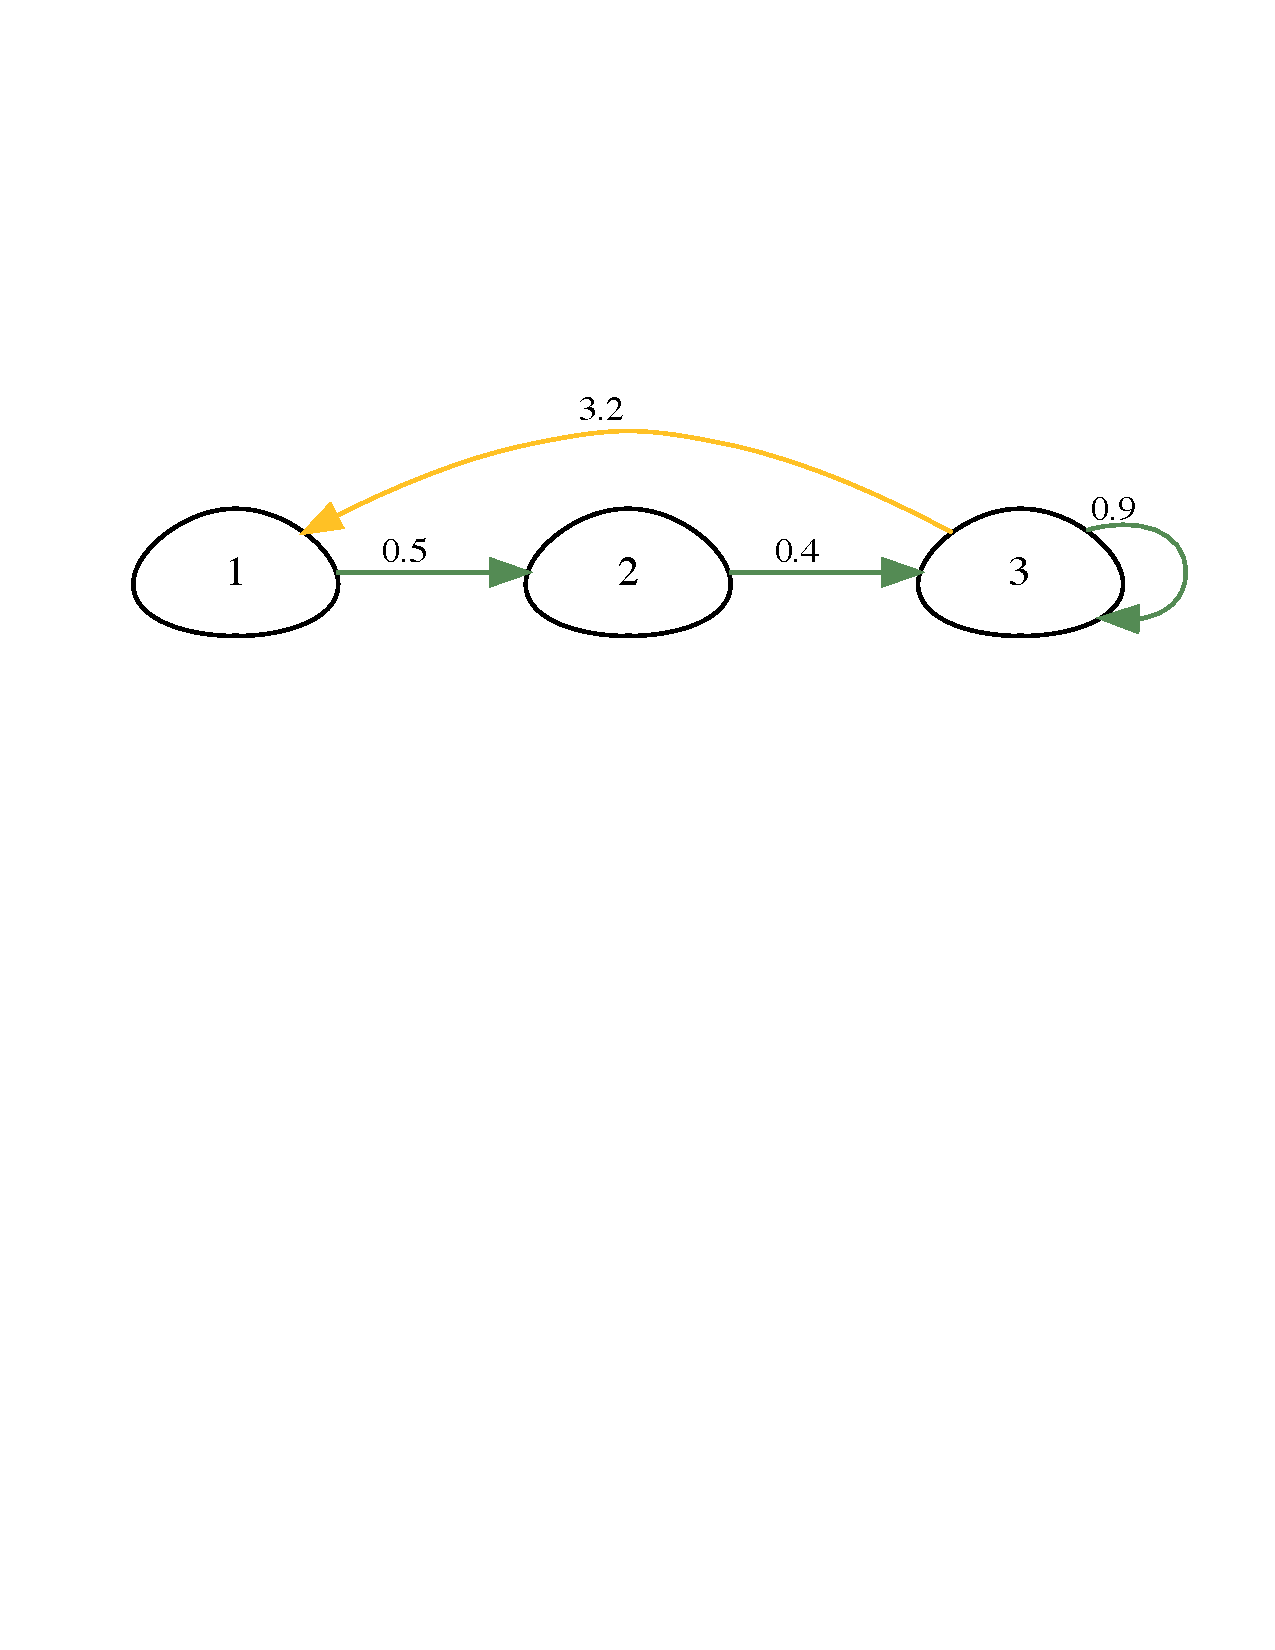
\includegraphics{121-Traduccion_protocolo_informacion_files/figure-pdf/Proto1-1.pdf}

\begin{center}\rule{0.5\linewidth}{0.5pt}\end{center}

\begin{enumerate}
\def\labelenumi{(\alph{enumi})}
\setcounter{enumi}{2}
\tightlist
\item
  Descripción del Censo
\end{enumerate}

\begin{table}
\fontsize{12.0pt}{14.0pt}\selectfont
\begin{tabular*}{\linewidth}{@{\extracolsep{\fill}}lr}
\toprule
Atributo del censo & Ejemplo \\ 
\midrule\addlinespace[2.5pt]
Duraci\\'on del Censo & May 2021 to May 2022 \\ 
Localidad & Sheffield, UK (53\textdegree24'41.5 N 1\textdegree30'02.3 W) \\ 
Intervalo de proyecci\\'on & 1 a\~no \\ 
Modo de reproducci\\'on & Pico de reproducci\\'on* (En Junio y Julio)\textsuperscript{\textit{1}} \\ 
Tipo de Censo & Pre-reproductivo \\ 
\bottomrule
\end{tabular*}
\begin{minipage}{\linewidth}
\textsuperscript{\textit{1}}Pico de reproducci\\'on = Birth-Pulse\\
\end{minipage}
\end{table}

\begin{center}\rule{0.5\linewidth}{0.5pt}\end{center}

\begin{enumerate}
\def\labelenumi{(\Alph{enumi})}
\setcounter{enumi}{3}
\tightlist
\item
  Nombres de las etapas y clasificación
\end{enumerate}

\begin{table}
\fontsize{12.0pt}{14.0pt}\selectfont
\begin{tabular*}{\linewidth}{@{\extracolsep{\fill}}lll}
\toprule
N\\'umero de las Etapas & Nombre de la Etapa & Critrio de Clasificaci\\'on \\ 
\midrule\addlinespace[2.5pt]
1 & Plantulas & Un individuo recientemente germinado que tiene menos de cuatro hojas y no ha desarrollado la estructura de roseta radial. El las hojas miden menos de tres cent\\'imetros de largo \\ 
2 & Rosetta & Un individuo con una morfolog\\'ia radial pronunciada en la estrucura de la hoja. Las hojas miden entre tres y seis cent\\'imetros en longitud \\ 
3 & Plantas adultas & Un individuo con una morfolog\\'ia radial pronunciada en la estrucura de la hoja. Las hojas miden m\\'as de seis cent\\'imetros en longitud \\ 
\bottomrule
\end{tabular*}
\end{table}

\begin{center}\rule{0.5\linewidth}{0.5pt}\end{center}

\begin{enumerate}
\def\labelenumi{(\Alph{enumi})}
\setcounter{enumi}{4}
\tightlist
\item
  Definiciones de las Tasas vitales
\end{enumerate}

\begin{longtable}[]{@{}
  >{\raggedright\arraybackslash}p{(\columnwidth - 4\tabcolsep) * \real{0.0803}}
  >{\raggedright\arraybackslash}p{(\columnwidth - 4\tabcolsep) * \real{0.7226}}
  >{\raggedright\arraybackslash}p{(\columnwidth - 4\tabcolsep) * \real{0.1971}}@{}}
\toprule\noalign{}
\begin{minipage}[b]{\linewidth}\raggedright
Tasa Vital
\end{minipage} & \begin{minipage}[b]{\linewidth}\raggedright
Definición
\end{minipage} & \begin{minipage}[b]{\linewidth}\raggedright
Provenencia de los valores
\end{minipage} \\
\midrule\noalign{}
\endhead
\bottomrule\noalign{}
\endlastfoot
\(S_{ij}\) & Supervivencia de la etapa \emph{j} a la etapa \emph{i} &
Datos de campo \\
\(N_{s}\) & Número de semillas por fruto & Datos de campo \\
\(N_{fx}\) & Número de frutos producido por un idividuo en el tamaño de
categoria \emph{x} & Datos de campo \\
\(P_{rx}\) & La probabilidad de reprodución de un adulto en la categoria
\emph{x} & Datos de campo \\
\(P_{s}\) & Probabilidad de germinación de semillas y supervivencia de
plantulas en el intervalo de proyección & Datos de Invernadero \\
\end{longtable}

\begin{enumerate}
\def\labelenumi{(\Alph{enumi})}
\setcounter{enumi}{5}
\tightlist
\item
  Valores de las razones de transición vitales
\end{enumerate}

\begin{longtable}[]{@{}
  >{\raggedright\arraybackslash}p{(\columnwidth - 6\tabcolsep) * \real{0.2192}}
  >{\raggedleft\arraybackslash}p{(\columnwidth - 6\tabcolsep) * \real{0.2192}}
  >{\raggedleft\arraybackslash}p{(\columnwidth - 6\tabcolsep) * \real{0.2329}}
  >{\raggedleft\arraybackslash}p{(\columnwidth - 6\tabcolsep) * \real{0.3288}}@{}}
\toprule\noalign{}
\begin{minipage}[b]{\linewidth}\raggedright
Etapas Vitales
\end{minipage} & \begin{minipage}[b]{\linewidth}\raggedleft
Estimados*
\end{minipage} & \begin{minipage}[b]{\linewidth}\raggedleft
Error Estandard**
\end{minipage} & \begin{minipage}[b]{\linewidth}\raggedleft
Tamaño de muestra (N)***
\end{minipage} \\
\midrule\noalign{}
\endhead
\bottomrule\noalign{}
\endlastfoot
\(S_{21}\) & 0.400 & 0.100 & 80 \\
\(S_{32}\) & 0.850 & 0.050 & 160 \\
\(S_{33}\) & 0.900 & 0.020 & 160 \\
\(N_{s}\) & 1000 & 150 & 80 \\
\(N_{f3}\) & 2.000 & 300 & 80 \\
\(P_{r3}\) & 0.300 & 0.040 & 200 \\
\(P_{s}\) & 0.005 & 0.001 & 500 \\
\end{longtable}

*Si estas estimaciones dependen del tamaño de la población (es decir,
dependencia de la densidad) o en respuesta a una variable ambiental (es
decir, ambiental, estocasticidad), la estimación debe comunicarse como
una función (por ejemplo,
\(S_{33}\sim\ 0,9\ +\ \beta_{precipitacion}\ \cdot\ 0,01\) donde la
precipitación ∼ N(5, 1)). Además, si se trata de una estimación puntual,
los investigadores deben indicar si los valores representan valores
medios o medianos.

**Esta medida de incertidumbre también puede ser la desviación estándar,
la varianza o un intervalo de confianza/creíble de la estimación, a
discreción. del investigador.

***Indique si la unidad de medida/replicación es a nivel de organismos
individuales o a nivel de grupos (por ejemplo, cohortes, colonias,
familias).

\begin{center}\rule{0.5\linewidth}{0.5pt}\end{center}

\begin{enumerate}
\def\labelenumi{(\Alph{enumi})}
\setcounter{enumi}{6}
\tightlist
\item
  Fórmula MPM (Mayo 2021 a Mayo 2022)
\end{enumerate}

\begin{longtable}[]{@{}lll@{}}
\toprule\noalign{}
Plantulas & Rosettas & Adultos \\
\midrule\noalign{}
\endhead
\bottomrule\noalign{}
\endlastfoot
0 & 0 & \(N_{s}*N_{f3}*P_{r3}*P{s}\) \\
\(S_{21}\) & 0 & 0 \\
0 & \(S_{32}\) & \(S_{33}\) \\
\end{longtable}

\begin{enumerate}
\def\labelenumi{(\Alph{enumi})}
\setcounter{enumi}{7}
\tightlist
\item
  Vector de la población (Mayo 2021)
\end{enumerate}

\begin{table}
\fontsize{12.0pt}{14.0pt}\selectfont
\begin{tabular*}{\linewidth}{@{\extracolsep{\fill}}rrr}
\toprule
Etapa & Cantidad & Intervalo de Confienza de 95\%* \\ 
\midrule\addlinespace[2.5pt]
1 & 1350 & 1150-1550 \\ 
2 & 550 & 530-570 \\ 
3 & 300 & 290-310 \\ 
\bottomrule
\end{tabular*}
\end{table}

*Esta medida de incertidumbre también puede ser la desviación estándar
de la estimación, la varianza o un intervalo de confianza/creíble a
discreción. del investigador.

3.6 \textbar{} Omitir etapas de vida crípticas

La identificación y estimación de tasas vitales en etapas crípticas
representa un reto en ecología de poblaciones. Se determinan las etapas
crípticas como puntos a lo largo del ciclo de vida de un organismo que
están, de una forma u otra, ocultos o se pasan por alto por ecologistas
de poblaciones al construir modelos de población (Doak, Diane Thomson \&
Jules, 2002). Una etapa de la vida puede ser críptica porque es
logísticamente difícil de observar, o, aunque si es observable, a su vez
es indistinguible de otra etapa (Nguyen et al., 2019). En las plantas,
etapas crípticas pueden surgir de los bancos de semillas, como en el
caso de las orquídeas, donde las semillas son demasiado pequeñas para
ser observadas e identificadas en el campo (Paniw et al., 2017) o
algunas perennes herbáceas (por ejemplo, \emph{Astragulus scaphoides})
donde períodos de latencia vegetativa permiten que los individuos
permanezcan escondidos bajo tierra durante una o más temporadas de
crecimiento (Gremer \& Sala, 2013). Además, los animales pueden exhibir
etapas crípticas al pasar por diapausa o retrasos en el desarrollo
debido a condiciones ambientales adversas (p.~ej. \emph{Aedes
albopictus}: Jia et al. (2016){]}. Aves marinas pelágicas (albatros,
petreles, pingüinos) a menudo pasan etapas pre-reproductivas en el mar,
a veces de duraciones de muchos años, y al ser así, se mantienen
completamente crípticas hasta volver a la colonia reproductora como
adultos. Métodos sofisticados de marcado-recaptura multi-estado pueden
proporcionar estimaciones de parámetros para estas partes del ciclo de
vida Choquet, Rouan \& Pradel (2009). Omitir una etapa críptica de la
vida puede reducir la realismo biológico de un MPM y alterar el número
de etapas en el MPM, que, en su conjunto puede impactar aún más los
resultados demográficos (Tenhumberg, Tyre \& Rebarber, 2009;
Salguero-Gómez \& Plotkin, 2010). En algunos casos, las etapas de la
vida crípticas solo se identificarán a través de un enfoque
multidisciplinario. incluyendo métodos de campo y de laboratorio, junto
con marcos bayesianos para integrar datos y conocimientos previos (por
ejemplo, Paniw et al., 2017).

3.7 \textbar{} Modelos de uno versus dos sexos

Gran parte de la demografía se centra en las hembras, bajo los supuestos
que la fertilidad está determinada por las hembras sin limitación por
los machos (ver Caswell, 2001, p. 568). Dichos modelos pueden incluir
machos (por ejemplo, Hunter et al., 2010), pero si la reproducción está
determinada por las tasas femeninas (es decir, dominado por la etapa de
hembras). Los machos representan un conjunto de etapas que no
contribuyen al crecimiento de la población. La mayoría de los MPM de
animales existentes están a base de hembras y femenino dominante
(Salguero-Gómez et al., 2016) dados sesgos de muestreo hacia mamíferos y
aves (Conde et al., 2019), a menudo no es factible, o necesario para la
pregunta de investigación, rastrear interacciones reproductivas
masculinas (Archer et al., 2022). Estos estudios, por lo general, asumen
una proporción de sexos 1:1, y las tasas vitales son congruente por sexo
y la reproducción no es limitada por los machos de la especie
(Compagnoni, Steigman \& Miller, 2017; Miller \& Compagnoni, 2022).
Mientras que un sexo los modelos son comunes en animales MPM'S
(actualmente 77\% en Comadre v. 4.21.8), se debe tener cuidado no hacer
suposiciones sobre la relación sexual dinámica dependiente dentro estos
sistemas (Archer et al., 2022). De hecho, estos supuestos no pueden ser
cumplido cuando cualquiera de los siguientes es cierto: que haya un
sesgo en la proporción de sexos (Archer et al., 2022), hay reproducción
sesgadas (Sky et al., 2022), o un alta sensibilidad de la dinámica de la
población en respuesta a la elección de apareamiento (Veran \&
Beissinger, 2009). Además, la detectabilidad de los diferentes sexos en
el muestreo dependiente del sexo puede confundir más las estimaciones de
la relación sexual y sus inpactos asociados sobre las tarifas vitales si
no se tiene en cuenta. Los modelos de dos sexos que no asumen la
dominancia por un sexo no son lineales y requiere especificaciones de
una función de apareamiento que describe la fertilidad en función del
macho y la abundancia hembras (Caswell, 2001). La definición de tales
funciones de apareamiento es generalmente difícil o imposible, excepto
en casos específicos como la estricta monogamia (Jenouvrier et al.,
2010).

Informar sobre las proporciones de sexos puede expandir enormemente el
alcance de un estudio Shyu \& Caswell (2016b); Por ejemplo, evaluar el
impacto de la razón de sexo cuando hay efecto Allee (Boukal \& Berec,
2002). Desafortunadamente, este tipo de análisis es raro y pocos
ejemplos son notado en la bases de datos de COMPADRE y COMADRE. Además,
si hay diferencias en los valores de la tasa vital entre sexos, como
supervivencia, crecimiento y/o producción reproductiva en los modelos
basado en un sexo solamente los MPM puede omitir procesos importantes
(Caswell, 2001, p. 568; Archer et al., 2022). En plantas, ejemplos de
investigaciones que incluye la dinámica de dos sexos raro (0.2\% en
COMPADRE v. 6.22.5). Este bajo porcentaje probablemente refleja en parte
la rareza de la plantas dioecía u otros sistemas de apareamiento con dos
o más sexos (Gabriel, John, et al., 2017) y los sistemas de apareamiento
polígamos que hace que la reproducción y la dinamica poblacional
limitado a los macho es raro (ver Compagnoni, Steigman \& Miller, 2017;
Miller \& Compagnoni, 2022).

3.8 \textbar{} Irreductibilidad y ergodicidad

Las propiedades de la irreductibilidad tiene implicaciones sobre la
diversidad de eigenvalue de una matriz y, por lo tanto, interpretaciones
biológicamente relevantes (e.g.~tasas de crecimiento de la población,
estructuras de etapa estable). Estas implicaciones son bien conocidos en
la literatura sobre MPM (Caswell, 2001). Matriz que son irreducible son
aquellas en la que el gráfico del ciclo de vida está completamente
conectado; es decir, existe una ruta directa o indirecta desde cualquier
etapa a cualquier otra etapa. A veces se afirma que los MPM reducibles
son de alguna manera inválido; ellos no son inválido. Hay (al menos)
cuatro situaciones en que matrices reducibles ocurren naturalmente.

Ciclos de vida con etapas post-reproductiva. Las etapas
post-reproductiva no pueden contribuir a la potencialmente reproductiva
(por ejemplo, MPM's para humanos, Orcas).

Modelos de dos sexos dominado por un sexo (generalmente mujeres, pero
podría ser hombre). En un modelo dominado por hembras, toda la
reproducción es acreditado a las mujeres. Los machos son producidos por
las hembras, pero los machos no hacen contribución a la parte femenina
del ciclo de vida por ejemplo, (Hunter et al., 2010) para osos polares).

Modelos espaciales en los que la dispersión es un direccional, como en
los sistemas fluviales (ríos) o corrientes oceánicas.

En los modelos de Edad × Etapas (Caswell, 2009; Caswell \&
Salguero-Gómez, 2013). En estos modelos, la reproducción produce (por
definición) individuos en la clase de edad 1, pero el modelo incluye
todo combinaciones de edad y etapa, incluidas combinaciones imposibles
de edad de clase 1 y etapas que no existen a los 1 años.

La reductibilidad puede o no ser fácil de detectar desde el gráfico del
ciclo de vida, pero se puede evaluar numéricamente. La matriz A es
irreducible si y solo si la matriz \(\left(I+A\right)^{s-1}\) es
positiva (Caswell, 2001). La irreductibilidad, junto con la
primitividad, es una condición suficiente para Ergodicidad, garantizando
que la población convergerá a la misma estructura estable
independientemente de la condición inicial. Una matriz reducible puede
no tener esta propiedad; claramente, por ejemplo, si una población
comenzó con un solo individuo post-reproductivo no convergerán a la
misma estructura que uno comenzó con algunos pre-reproductivos
individuos. Con respecto a la ergodicidad, también se sabe que un MPM es
ergódico si y solo si todas las entradas de su vector propio dominante
izquierdo (v) son positivos (Stott et al., 2010). En resumen, a pesar
del modelo apropiado estructura y parametrización correcta, los datos
demográficos pueden conducir a matrices reducibles y/o no ergódico.

4 \textbar{} Representación completa de un MPM en publicaciones

En esta sección, justificamos la necesidad de una presentación clara de
MPM's en la literatura científica, sugerencias dónde archivar los MPM's
en base da datos de acceso abierto, y discutir cómo estas dos acciones
benefician a los autores, revista editorial, lectores, demógrafos
comparativos, meta-analistas y la disciplina en general. Una tabla que
contiene la lista de los datos a incluir al publicar MPM's junto con una
justificación para la inclusión. Se pueden encontrar ejemplos de buenas
prácticas en Tabla S1.

4.1 \textbar{} Partición de los procesos demográficos

Es importante definir a que se refiere cada elemento de una matriz de un
MPM's. Varios procesos demográficos pueden superponerse al mismo
elemento matriz en un MPM, particularmente en especies con un rápido y/o
variable ciclo de vida relativo a los intervalos de proyección del MPM.
Por ejemplo, el parámetro en un MPM que representa el enlace entre
individuos grandes en el tiempo \(t\) y individuos más pequeños en el
tiempo \(t+1\) podría corresponder a la reproducción sexual,
reproducción clonal, fisión, retroceso o un conjunto de los procesos
anteriores. Las derivaciones matemáticas de parámetros clave de la
historia de vida (por ejemplo, generación el tiempo, la esperanza de
vida, la tasa de senescencia, el grado de iteroparidad) requieren que
estos procesos están claramente separados (Jones et al., 2022). Esto
separaciones es crítica para la familia de análisis basados en las
cadenas de Markov; la matriz U define las transiciones de estado
transitorio en un análisis de Chain de Markov absorbente (Caswell, 2011;
Caswell \& Salguero-Gómez, 2013). Claramente describiendo la estructura
subyacente de las tasas demográficas en un diagrama del ciclo de vida y
su consecuente modelo de población de la matriz completa A, se puede
separar matrices en los procesos de supervivencia (por ejemplo,
progresión/crecimiento, retroceso/ contracción, fisión, fusión, estasis)
en la submatriz U, una matriz de reproducción sexual en el submatriz F y
la reproducción clonal en la submatriz C (Figura 4). Es importante
destacar que tanto que las matrices de F y C incluye elementos que deben
incorporar la supervivencia de acuerdo con el tipo de censo (es decir,
pre-/post-reproductivo censo).

Informando claramente la matriz A y las submatrices U, F y C se lleva
dos beneficios clave: (1) indica explícitamente cómo se generan los
valores de la matriz A de tasas vitales subyacentes; y (2) los
submatrices pueden ser utiliza para calcular una gran gran cantidad de
medidas demográficas que no pueden calcularse a partir de solamente la
matriz A, como la longevidad (promedio y varianza), tiempos de ocupación
(promedio y variaciones), la distribución de la reproductiva de por vida
de los individuos (promedio y variaciones), taza de reproducción neta,
tiempo de generación y entropía (KeyFitz Entropy (Keyfitz, 1968) y la
entropía de Demetrius (Demetrius, 1992) entre otros.

4.2 \textbar{} Atribución de fuentes de datos secundarias

Las fuentes de datos secundarias son críticas para la reproducibilidad.
Las fuentes de datos proporcionan información y soporte para las
metodologías utilizadas en la construcción MPM. En algunos casos, los
MPM simplemente usan datos secundarios para estimar algunos parámetros
del ciclo de vida, mientras que otros se construyen puramente de fuentes
secundarias (ver Tabla S1). Las fuentes secundarias incluyen estudios
previos, datos de bases de datos, simulaciones, observaciones indirectas
y estimaciones teóricas. El uso de fuentes de datos secundarias puede
significar que el MPM final no representa con precisión las tasas de
razón vitales, y así debe reconocerse en la sección de métodos de la
publicación o su información de apoyo. La comunicación de fuentes
secundarias debería ser suficiente para determinar su proveniencia e
incluye la fuente de los datos, si se estimó un punto, el intervalo de
confianza o la distribución y como se integró con la fuente de datos
primaria, así como la justificación de su inclusión. Por ejemplo,
(Omeyer et al., 2021) presenta una tabla de fuentes de datos utilizadas
en la construcción de MPM. Si estas fuentes secundarias no se reconocen
en conjunto con el MPM, los inferidos procesos demográficos, por
realista que sean, pueden no pasar revisión por pares ni aceptada de la
comunidad científica. A su vez, la comunicación clara de estas fuentes
secundarias es muy recomendable.


\includegraphics{Figures/Matrices_A_U_F_C.jpg}

4.3 \textbar{} Archivando los datos en COMPADRE y COMADRE

Proponemos que las bases de datos de la matriz de COMPADRE y COMADRE
proporcione la forma más adecuada de archivar y acceder a MPM's.
Mientras reconocemos que hay otros repositorios de bases de datos
ecológicas (por ejemplo, Dryad: \url{https://datadryad.org/}; figshare:
\url{https://figshare.com}; Zenodo: \url{https://zenodo.org}), la base
de datos de COMPADRE COMADRE de acceso abierto
(\url{https://compadre-db.org/Contribute}) proporciona una plataforma de
archivo de datos dedicada, específicamente para MPM's, que permite
contribuciones directas de los investigadores y la digitalización de MPM
publicados por nuestros equipos de validación de datos. La integración
de un portal usando una pagina web para la entrada de datos proporciona
un proceso de curación de datos estructurado (es decir, desde la
detección, la estandarización, hasta la validación) que pueden acomodar
MPM de diferentes dimensiones y diversas historias de vida. Al ingresar,
los MPM se complementan con variables biogeográfico relevante y detalles
sobre la metodología del censo en COMPADRE y COMADRE. Detalles de la
publicación original, incluyendo doi y citas funcional (ver
\url{https://compadre-db.org/Education/article/obtaining-references}
donde se almacenan junto con cada MPM para garantizar que su
contribución a cualquier publicación futura es reconocida. Todos los
datos están archivados a largo plazo a través de Oxford Open Access y
con apoyo de la Biblioteca Bodleian.

Otras mejoras recientes integradado a COMPADRE y COMADRE ayudará aún más
a la comunidad de cientfica. Anteriormente, las bases de datos solo eran
accesibles a través de la descarga de un archivo R-Object que contenía
todas las matrices en esa versión de la base de datos. La base de datos
es ahora accesible a través de un sitio web
(\url{https://compadre-db.org/QueryDatabase}) que permite a los usuarios
encontrar y descargar matrices individuales. También nos esforzamos por
empoderar a los investigadores y educadores con materiales de enseñanza
(\url{https://compadre-db.org/Education}) y la producción de nuevos
paquetes R (Jones et al., 2022) para facilitar escalabilidad de MPM
investigación. Junto con estos materiales, todos los detalles de la
estructura de la base de datos y el flujo de trabajo son de acceso libre
(\url{https://jonesor.github.io/CompadreGuides/user-guide.html}). Estas
mejoras en las bases de datos y su estructura de interfaz ha sido
directamente dirigido a equipar a los demógrafos con más herramientas
para realizar investigaciones y capacitar a los estudiantes en MPM's
junto con el mejoras en transparencia de la base de datos para
garantizar buenas prácticas en la investigación.

5 \textbar{} Un protocolo estandarizado para reportar MPM's

Aquí presentamos una lista de verificación propuesta sobre cómo reportar
un MPM en publicaciones (Recuadro 1). Recomendamos utilizar la lista de
verificación cuando diseñar la recopilación de datos, así como al
redactar el MPM para publicación. Recomendamos utilizar esta plantilla
como apoyo de la información necesaria para los MPM ya que permite una
comunicación clara de la construcción de los modelos además de la
facilidad para integrar publicaciones MPM a las bases de datos COMPADRE
y COMADRE.

6 \textbar{} La teoría non es estática: la no linealidad, dependencia
del medio ambiente y los modelos de múltiple estados.

Los MPM se han convertido en un enfoque predominante en la lista de
herramientas en el estudio de ecología de población en parte debido a su
simplicidad de construcción y análisis. Pero la teoría subyacente basada
en matrices para estudiar demografía no se detiene y en los últimos 20
años ha aumentado espectacularmente. Estos nuevos métodos producen
modelos cuya estructura no se ajusta en los marcos para la presentación
de informes que parecían tan completos en el pasado. Estos avances
recientes en la teoría y los métodos de MPM permiten investigadores
vincular la dinámica demográfica y el efecto del medio ambiente sobre la
demografía y múltiples rasgos individuales (por ejemplo, sexo y edad)
(Childs, Sheldon \& Rees, 2016); edad y parentesco (Caswell, 2019a,
2020) en lugar de un solo rasgo de la especie. Estos avances también
ofrecen beneficios para el estudio de respuestas de la población al
clima extremo (Jenouvrier et al., 2022), en adición de investigaciones
demográfica más matizadas de aspectos comparativos y evolutivos (Childs,
Sheldon \& Rees, 2016). En esta sección repasamos algunas áreas
interesantes de demografía estructurada que pueden abrir nuevas
preguntas de investigación para el demógrafo y enumerar algunas de las
desafíos que plantean para la comunicación y la presentación de
informes.

6.1 \textbar{} Modelos no lineal

Los MPM no lineales son aquellos en los que las entradas de la matriz de
proyección dependen del estado de la población (números y estructura) y
pueden ser influenciado por la frecuencia o la densidad
denso-dependiente. Los modelos que son influenciado por la densidad de
frecuencia no lineal dependen sólo de la relativa abundancia de etapas;
ellos ocurren en los modelos de dos sexos en los que el apareamiento
depende de la relación abundancia de machos y hembras, y en modelos
genéticos de poblaciones donde la dinámica depende de la abundancia
relativa de genotipos (Vries \& Caswell, 2019). Los modelos
denso-dependiente dependen de la abundancia y estructura de la
población; ejemplos recientes incluyen a (Pardini et al., 2009) y (Shyu
et al., 2013) para análisis de estrategias de control de la mostaza con
ajo \emph{Alliaria petiolata} y de (Vries \& Caswell, 2019) para
estudios de laboratorio de resistencia a pesticidas en \emph{Tribolium}.

Los análisis de MPM no lineales se centra en los resultados demográficos
diferentes a los de los modelos lineales; equilibrios, atractores,
bifurcaciones, oscilaciones y estabilidad Cushing (2003). Sin embargo,
¿qué hace que estos modelos sean problemáticos para la situación actual?
El estatus de COMPADRE y COMADRE es que la unidad del modelo no es una
matriz, sino más bien una función matricial, en la que las entradas de
la matriz de proyección son funciones del estado de la población. Los
análisis de sensibilidad están disponibles para estudiar prácticamente
cualquier grupo demográfico resultado en respuesta a cualquier parámetro
(Caswell, 2019b), pero informar las funciones que definen el MPM no lo
es en absoluto estandarizado.

6.1 \textbar{} Dependencia del Ambiente

Un problema similar surge en entornos dependientes del medio ambiente.
En algunos modelos, algunas o todas las tasas demográficas son funciones
de algunos aspectos del medio ambiente; por ejemplo, los osos polares
como funciones de los parámetros estadísticas del hielo marino del
Ártico (Regehr et al., 2010), los sifaka de Madagascar como funciones de
lluvia (Lawler et al., 2009), el pingüino emperador en función de los
patrones estacionales del hielo marino en la Antártida (Jenouvrier et
al., 2012) y la ballena franca del Atlántico norte en función del tiempo
y de las tendencias en el tiempo (Fujiwara \& Caswell, 2001). Al igual
que con los MPM no lineales, el modelo no es una matriz, sino una
función que se mapea desde las variable(s) ambientales a las entradas de
la matriz. Los protocolos para informar dichas funciones aún no están
disponibles pero es importante desarrollarlas.

6.3 \textbar{} Modelos de múltiples estados

Un área emergente en la investigación demográfica es la construcción y
análisis de MPM multiestatales, en los que se clasifican los individuos
por más de una variable de estado. Esto incluye edad y etapa. (Caswell
\& Salguero-Gómez, 2013), escenario y localización espacial (Hunter \&
Caswell, 2005), estadio y genotipo (Vries \& Caswell, 2019), estadio y
estado de infección (Klepac \& Caswell, 2011), edad y heterogeneidad no
medida (Hartemink, Missov \& Caswell, 2017) y etapas específicas de
incidencia de enfermedades (Caswell \& Daalen, 2021). Una presentación
detallada de los métodos se se encuentra en (Caswell et al., 2018) y la
extensión a más de dos ejes estatales (los llamados matrices de
hiperestado) se proporciona en (Roth \& Caswell, 2016). La incorporación
de estados adicionales permite a los investigadores separar varias
fuentes de información individual de heterogeneidad, la varianza en la
historia de vida de los individuos del mismo modelo poblacional y sus
resultados, en adición de plantear comparaciones más profundas y
preguntas evolutivas. Por ejemplo, la edad materna tiene un fuerte
impacto en las tasas vitales en rotíferos monogonones (Bock et al.,
2019). Aplicando métodos de permutación-vec (Caswell, 2012) para
construir MPM multi-estatales han permitido a los investigadores
cuantificar el nivel de población impactos del efecto observado de la
edad materna e investigar los procesos evolutivos que pueden conducir a
este tipo de senescencia en rotíferos (Hernández et al., 2020). MPM
multidimensionales y los métodos de la cadena de Markov han sido
particularmente importantes en el estudio de la ``suerte'' en las
historias de vida, que explora por qué algunos individuos viven mucho
tiempo y prosperan, mientras que otros no (Snyder \& Ellner, 2022). En
estudios de ``suerte'', la variación entre individuos en la historia de
vida se divide en contribuciones de la variación entre grupos y dentro
del grupo por ejemplo, (Daalen \& Caswell, 2017; Snyder \& Ellner,
2018). Ejemplos de fuentes de heterogeneidad individual incluyen edad
materna (Daalen et al., 2022), año de nacimiento ambiente (Snyder \&
Ellner, 2022) y variación genética (Steiner, Tuljapurkar \& Roach,
2021). El efecto de la variación dentro se llama estocasticidad
individual o ``suerte'' y surge del hecho de que las tasas vitales son
procesos probabilísticos.

Estos modelos plantean un desafío para la presentación de informes
porque el MPM no consta de una única matriz, sino de cuatro conjuntos de
matrices. Considerar un modelo clasificado como edad × etapa. Esos
modelos son compuesto por un conjunto de matrices dando transiciones
entre etapas para cada clase de edad, un conjunto de matrices D
asignando transiciones de edad para cada etapa y un conjunto de matrices
F que asignan transiciones de edad específicas para cada etapa de
fecundidad, y un conjunto de matrices H que asignan crías recién nacidas
a las edades apropiadas. Estos están ensamblados en matrices de
transición y fertilidad estructuradas en bloques a partir de las cuales
todos los resultados demográficos habituales se pueden calcular y
relacionar con tanto la edad como la etapa (por ejemplo, ver Caswell \&
Salguero-Gómez, 2013 para un análisis de gradientes de selección tanto
para edad como para tamaño).

7 \textbar{} Discusión

La investigación demográfica ha avanzado mucho desde la introducción de
los estudios demográficos a base de edad (Leslie, 1945) y modelos
matriciales basado en etapas (Lefkovitch, 1965). Los avances en este
campo se han visto impulsados en parte mediante una comunicación clara
de los métodos y el código asociado. Deseamos continuar expandir el uso
de esas herramientas con la comunicación de MPM.

A medida que la profundidad y amplitud de la literatura continúa
expandiéndose, estamos empezando a construir una imagen integral de la
demografía y explorar el espectro de la vida biologica (Adler et al.,
2014; Salguero-Gomez et al., 2017; Healy et al., 2019). A través de la
base de datos de COMPADRE y COMADRE, hemos llegado a apreciar la
utilidad y oportunidades de una forma estandarizada de compilar MPM. De
hecho, una parte importante del tiempo (\textgreater50\%) que dedicamos
a curar estas bases de datos en realidad no se trata de digitalización,
verificación de errores, y complementar datos, sino en contactar a los
autores para obtener aclaraciones y solicitud de datos y metadatos
faltantes. A través de este arduo proceso, hemos identificado valiosas
información en MPM que no estaba en las publicaciones originales. Si
bien los datos faltantes se destacan aquí como particularmente
importante y refleja principalmente los intereses y perspectivas de
demógrafos comparativos, incluidos los datos descritos en el métodos
estandarizado qué beneficiaría a la demografía en su conjunto.

Este artículo pretende actuar como una referencia útil para autores,
editores, revisores, gestores/conservacionistas y demógrafos
comparativos. Además, esperamos que este manuscrito promueva una
discusión constructiva sobre el propósito, la construcción y la
presentación de información demográfica a base de etapas. El cuadro 1
contiene un ejemplo completo de la información clave que creemos que
debería incorporarse a la publicación de cualquier MPM. Al adoptarse los
métodos que se sugiere aquí, habrá claros beneficios para el crecimiento
de las bases de datos demográficas COMPADRE y COMADRE; sin embargo,
creemos que estos beneficios se extienden más allá de COMPADRE y
usuarios de COMADRE hacia todo el campo de la ecología de poblaciones y
campos que utilizan MPM para su propia beneficio (por ejemplo,
conservación biología y monitoreo de la biodiversidad). Un mayor nivel
de detalle y transparencia al describir cómo y por qué se produce un MPM
dará como resultado una mayor precisión, accesibilidad, reproducibilidad
y citabilidad; eso tiene claros beneficios para el campo en su conjunto
y para los investigadores. Además, una mayor coherencia y transparencia
facilita la revisión por pares y, de hecho, estas directrices pueden
ofrecer una herramienta que puede ser citada por editores asociados y
revisores por pares y puede ser recomendado como guia para los pasos
sugeridos aquí. Además, la adopción de los pasos sugeridos aquí puede
aumentar confianza en los resultados presentados y facilitar el
aprendizaje/adopción de MPM por investigadores que inician su carrera.

Finalmente, cerramos con una precaución. Hemos utilizado el término
``preciso'' en puntos a lo largo de este documento, aplicados a los MPM,
pero debemos reconocer que no existe un modelo exacto, ya sea un MPM o
cualquier otro tipo. Un modelo es una serie de selección de parámetros,
selección de aspectos o variables que se incluyen y otros que no se
incluye. La selección de modelos como técnicas de selección como AIC
(Akaike Information Criterion; (Anderson \& Burnham, 2002) hacen estas
opciones explícitas y miden su apoyo en términos de probabilidad. Pero
incluso sin utilizar el método estadístico explícito, el mensaje es
claro. La opciones de ``i''-estado/variables, de intervalos de
proyección, de tipos de variación temporal, de dependencia funcional de
un conjunto elegido de factores ambientales, etc., todos ellos son
inexactos. La cuestión no es buscar la precisión: es ser claro al
comunicar las decisiones que tomó al construir el modelo, los análisis
usted eligió aplicar y la interpretación de los resultados. Una modelo
`precisa' de un sistema ecológico, experimental u observacional sería
tan complicado como un sistema real. Eso no termina bien (Borges, 1999).

Supporting Information

Additional supporting information can be found online in the Supporting
Information section at the end of this article. Data S1: A survey on
matrix communication.

\phantomsection\label{refs}
\begin{CSLReferences}{1}{0}
\bibitem[\citeproctext]{ref-adler2014functional}
Adler PB, Salguero-Gómez R, Compagnoni A, Hsu JS, Ray-Mukherjee J,
Mbeau-Ache C, Franco M. 2014. Functional traits explain variation in
plant life history strategies. \emph{Proceedings of the National Academy
of Sciences} 111:740--745.

\bibitem[\citeproctext]{ref-anderson2002avoiding}
Anderson DR, Burnham KP. 2002. Avoiding pitfalls when using
information-theoretic methods. \emph{The Journal of Wildlife
Management}:912--918.

\bibitem[\citeproctext]{ref-archer2022sex}
Archer CR, Paniw M, Vega-Trejo R, Sepil I. 2022. A sex skew in
life-history research: The problem of missing males. \emph{Proceedings
of the Royal Society B} 289:20221117.

\bibitem[\citeproctext]{ref-baudisch2013pace}
Baudisch A, Salguero-Gómez R, Jones OR, Wrycza T, Mbeau-Ache C, Franco
M, Colchero F. 2013. The pace and shape of senescence in angiosperms.
\emph{Journal of Ecology} 101:596--606.

\bibitem[\citeproctext]{ref-beissinger1998use}
Beissinger SR, Westphal MI. 1998. On the use of demographic models of
population viability in endangered species management. \emph{The Journal
of Wildlife Management}:821--841.

\bibitem[\citeproctext]{ref-bernard2023mosaic}
Bernard C, Santos GS, Deere JA, Rodriguez-Caro R, Capdevila P, Kusch E,
Gascoigne SJ, Jackson J, Salguero-Gómez R. 2023. MOSAIC-a unified trait
database to complement structured population models. \emph{Scientific
Data} 10:335.

\bibitem[\citeproctext]{ref-bock2019maternal}
Bock MJ, Jarvis GC, Corey EL, Stone EE, Gribble KE. 2019. Maternal age
alters offspring lifespan, fitness, and lifespan extension under caloric
restriction. \emph{Scientific Reports} 9:3138.

\bibitem[\citeproctext]{ref-borges1999collected}
Borges JL. 1999. \emph{Collected fictions}. Penguin.

\bibitem[\citeproctext]{ref-boukal2002single}
Boukal DS, Berec L. 2002. Single-species models of the allee effect:
Extinction boundaries, sex ratios and mate encounters. \emph{Journal of
Theoretical Biology} 218:375--394.

\bibitem[\citeproctext]{ref-bruijning2019demographic}
Bruijning M, Jongejans E, Turcotte MM. 2019. Demographic responses
underlying eco-evolutionary dynamics as revealed with inverse modelling.
\emph{Journal of Animal Ecology} 88:768--779.

\bibitem[\citeproctext]{ref-buckley2010causes}
Buckley YM, Ramula S, Blomberg SP, Burns JH, Crone EE, Ehrlén J, Knight
TM, Pichancourt J-B, Quested H, Wardle GM. 2010. Causes and consequences
of variation in plant population growth rate: A synthesis of matrix
population models in a phylogenetic context. \emph{Ecology {L}etters}
13:1182--1197.

\bibitem[\citeproctext]{ref-capdevila2020towards}
Capdevila P, Stott I, Beger M, Salguero-Gómez R. 2020. Towards a
comparative framework of demographic resilience. \emph{Trends in
{E}cology \& {E}volution} 35:776--786.

\bibitem[\citeproctext]{ref-caswell2001matrix}
Caswell H. 2001. \emph{Matrix {P}opulation {M}odels: Construction,
analysis, and interpretation}. Sunderland, Massachusetts, USA: Sinauer
Associates.

\bibitem[\citeproctext]{ref-caswell2009stage}
Caswell H. 2009. Stage, age and individual stochasticity in demography.
\emph{Oikos} 118:1763--1782.

\bibitem[\citeproctext]{ref-caswell2011beyond}
Caswell H. 2011. Beyond r 0: {D}emographic models for variability of
lifetime reproductive output. \emph{PloS One} 6:e20809.

\bibitem[\citeproctext]{ref-caswell2012matrix}
Caswell H. 2012. Matrix models and sensitivity analysis of populations
classified by age and stage: A vec-permutation matrix approach.
\emph{Theoretical Ecology} 5:403--417.

\bibitem[\citeproctext]{ref-Caswell_41_24}
Caswell H. 2019a. {The formal demography of kinship: A matrix
formulation}. \emph{Demographic Research} 41:679--712. DOI:
\href{https://doi.org/10.4054/DemRes.2019.41.24}{10.4054/DemRes.2019.41.24}.

\bibitem[\citeproctext]{ref-caswell2019sensitivity}
Caswell H. 2019b. \emph{Sensitivity analysis: Matrix methods in
demography and ecology}. Springer Nature.

\bibitem[\citeproctext]{ref-caswell2020formal}
Caswell H. 2020. The formal demography of kinship ii. \emph{Demographic
Research} 42:1097--1144.

\bibitem[\citeproctext]{ref-caswell1998harbor}
Caswell H, Brault S, Read AJ, Smith TD. 1998. Harbor porpoise and
fisheries: An uncertainty analysis of incidental mortality.
\emph{Ecological Applications} 8:1226--1238.

\bibitem[\citeproctext]{ref-caswell2021healthy}
Caswell H, Daalen S van. 2021. Healthy longevity from incidence-based
models. \emph{Demographic Research} 45:397--452.

\bibitem[\citeproctext]{ref-caswell2013age}
Caswell H, Salguero-Gómez R. 2013. Age, stage and senescence in plants.
\emph{Journal of Ecology} 101:585--595.

\bibitem[\citeproctext]{ref-caswell2018age}
Caswell H, Vries C de, Hartemink N, Roth G, Daalen SF van. 2018.
Age\(\times\) stage-classified demographic analysis: A comprehensive
approach. \emph{Ecological Monographs} 88:560--584.

\bibitem[\citeproctext]{ref-che2021comparative}
Che-Castaldo J, Havercamp K, Watanuki K, Matsuzawa T, Hirata S, Ross SR.
2021. Comparative survival analyses among captive chimpanzees (\emph{pan
{t}roglodytes}) in america and japan. \emph{PeerJ} 9:e11913.

\bibitem[\citeproctext]{ref-che2020comments}
Che-Castaldo J, Jones OR, Kendall BE, Burns JH, Childs DZ, Ezard TH,
Hernandez-Yanez H, Hodgson DJ, Jongejans E, Knight T, others. 2020.
Comments to {``persistent problems in the construction of matrix
population models.''}

\bibitem[\citeproctext]{ref-childs2016evolution}
Childs DZ, Sheldon BC, Rees M. 2016. The evolution of labile traits in
sex-and age-structured populations. \emph{Journal of Animal Ecology}
85:329--342.

\bibitem[\citeproctext]{ref-choquet2009program}
Choquet R, Rouan L, Pradel R. 2009. Program e-SURGE: A software
application for fitting multievent models. \emph{Modeling demographic
processes in marked populations}:845--865.

\bibitem[\citeproctext]{ref-clubb2003captivity}
Clubb R, Mason G. 2003. Captivity effects on wide-ranging carnivores.
\emph{Nature} 425:473--474.

\bibitem[\citeproctext]{ref-clubb2009fecundity}
Clubb R, Rowcliffe M, Lee P, Mar KU, Moss C, Mason GJ. 2009. Fecundity
and population viability in female zoo elephants: Problems and possible
solutions. \emph{Animal Welfare} 18:237--247.

\bibitem[\citeproctext]{ref-compagnoni2017can}
Compagnoni A, Steigman K, Miller TE. 2017. Can't live with them, can't
live without them? Balancing mating and competition in two-sex
populations. \emph{Proceedings of the Royal Society B: Biological
Sciences} 284:20171999.

\bibitem[\citeproctext]{ref-conde2019data}
Conde DA, Staerk J, Colchero F, Silva R da, Schöley J, Baden HM, Jouvet
L, Fa JE, Syed H, Jongejans E, others. 2019. Data gaps and opportunities
for comparative and conservation biology. \emph{Proceedings of the
National Academy of Sciences} 116:9658--9664.

\bibitem[\citeproctext]{ref-cooch2003apparent}
Cooch EG, Gauthier G, Rockwell RF. 2003. Apparent differences in
stochastic growth rates based on timing of census: A cautionary note.
\emph{Ecological Modelling} 159:133--143.

\bibitem[\citeproctext]{ref-coulson2001age}
Coulson T, Catchpole EA, Albon SD, Morgan BJ, Pemberton J, Clutton-Brock
TH, Crawley M, Grenfell BT. 2001. Age, sex, density, winter weather, and
population crashes in soay sheep. \emph{Science} 292:1528--1531.

\bibitem[\citeproctext]{ref-cushing2003chaos}
Cushing JM. 2003. \emph{Chaos in ecology: Experimental nonlinear
dynamics}. Elsevier.

\bibitem[\citeproctext]{ref-van2017lifetime}
Daalen SF van, Caswell H. 2017. Lifetime reproductive output: Individual
stochasticity, variance, and sensitivity analysis. \emph{Theoretical
Ecology} 10:355--374.

\bibitem[\citeproctext]{ref-van2022contributions}
Daalen SF van, Hernández CM, Caswell H, Neubert MG, Gribble KE. 2022.
The contributions of maternal age heterogeneity to variance in lifetime
reproductive output. \emph{The American Naturalist} 199:603--616.

\bibitem[\citeproctext]{ref-davis2022managed}
Davis KJ. 2022. Managed culls mean extinction for a marine mammal
population when combined with extreme climate impacts. \emph{Ecological
Modelling} 473:110122.

\bibitem[\citeproctext]{ref-de2009database}
De Magalhaes J, Costa. 2009. A database of vertebrate longevity records
and their relation to other life-history traits. \emph{Journal of
evolutionary biology} 22:1770--1774.

\bibitem[\citeproctext]{ref-demetrius1992growth}
Demetrius L. 1992. Growth rate, population entropy, y evolutionary
dynamics. \emph{Theoretical Population Biology} 41:208--236.

\bibitem[\citeproctext]{ref-doak2002population}
Doak DF, Diane Thomson, Jules ES. 2002. \emph{Population viability
analysis for plants: Understanding the demographic consequences of seed
banks for population health}. University of Chicago Press.

\bibitem[\citeproctext]{ref-doak2005correctly}
Doak DF, Morris WF, Pfister C, Kendall BE, Bruna EM. 2005. Correctly
estimating how environmental stochasticity influences fitness and
population growth. \emph{The American Naturalist} 166:E14--E21.

\bibitem[\citeproctext]{ref-ebert1999demography}
Ebert thomas A. 1999. \emph{Plant and {A}nimal {P}opulations. {M}ethods
in {D}emography}. Academic Press.

\bibitem[\citeproctext]{ref-ellner2016data}
Ellner SP, Childs DZ, Rees M, others. 2016. Data-driven modelling of
structured populations. \emph{A practical guide to the Integral
Projection Model. Cham: Springer}.

\bibitem[\citeproctext]{ref-emery2005effects}
Emery SM, Gross KL. 2005. Effects of timing of prescribed fire on the
demography of an invasive plant, spotted knapweed \emph{{C}entaurea
{m}aculosa}. \emph{Journal of Applied Ecology} 42:60--69.

\bibitem[\citeproctext]{ref-ezard2010matrix}
Ezard TH, Bullock JM, Dalgleish HJ, Millon A, Pelletier F, Ozgul A,
Koons DN. 2010. Matrix models for a changeable world: The importance of
transient dynamics in population management. \emph{Journal of Applied
Ecology} 47:515--523.

\bibitem[\citeproctext]{ref-ferreira2016marsupial}
Ferreira MS, Kajin M, Cerqueira R, Vieira MV. 2016. Marsupial population
dynamics in a tropical rainforest: Intraspecific competition and
nonlinear effect of rainfall. \emph{Journal of Mammalogy} 97:121--127.

\bibitem[\citeproctext]{ref-franco1996life}
Franco M, Silvertown J. 1996. Life history variation in plants: An
exploration of the fast-slow continuum hypothesis. \emph{Philosophical
Transactions of the Royal Society of London. Series B: Biological
Sciences} 351:1341--1348.

\bibitem[\citeproctext]{ref-fujiwara2001demography}
Fujiwara M, Caswell H. 2001. Demography of the endangered north atlantic
right whale. \emph{Nature} 414:537--541.

\bibitem[\citeproctext]{ref-gabriel2017rarity}
Gabriel A, John R, others. 2017. On the rarity of dioecy in flowering
plants. \emph{Molecular Ecology} 26.

\bibitem[\citeproctext]{ref-gascoigne2023standard}
Gascoigne SJ, Rolph S, Sankey D, Nidadavolu N, Stell Pičman AS,
Hernández CM, Philpott ME, Salam A, Bernard C, Fenollosa E, others.
2023. A standard protocol to report discrete stage-structured
demographic information. \emph{Methods in Ecology and Evolution}
14:2065--2083.

\bibitem[\citeproctext]{ref-gerstner2017will}
Gerstner K, Moreno-Mateos D, Gurevitch J, Beckmann M, Kambach S, Jones
HP, Seppelt R. 2017. Will your paper be used in a meta-analysis? Make
the reach of your research broader and longer lasting. \emph{Methods in
Ecology and Evolution} 8:777--784.

\bibitem[\citeproctext]{ref-gontijo2020using}
Gontijo LM, Carvalho RM. 2020. Using life stage-structured matrix models
to determine natural enemy: Pest release ratios for augmentative
biological control. \emph{Journal of Applied Entomology} 144:364--372.

\bibitem[\citeproctext]{ref-gremer2013risky}
Gremer JR, Sala A. 2013. It is risky out there: The costs of emergence
and the benefits of prolonged dormancy. \emph{Oecologia} 172:937--947.

\bibitem[\citeproctext]{ref-gurevitch2018meta}
Gurevitch J, Koricheva J, Nakagawa S, Stewart G. 2018. Meta-analysis and
the science of research synthesis. \emph{Nature} 555:175--182.

\bibitem[\citeproctext]{ref-hartemink2017stochasticity}
Hartemink N, Missov TI, Caswell H. 2017. Stochasticity, heterogeneity,
and variance in longevity in human populations. \emph{Theoretical
Population Biology} 114:107--116.

\bibitem[\citeproctext]{ref-healy2019animal}
Healy K, Ezard TH, Jones OR, Salguero-Gómez R, Buckley YM. 2019. Animal
life history is shaped by the pace of life and the distribution of
age-specific mortality and reproduction. \emph{Nature Ecology \&
Evolution} 3:1217--1224.

\bibitem[\citeproctext]{ref-hernandez2020demographic}
Hernández CM, Daalen SF van, Caswell H, Neubert MG, Gribble KE. 2020. A
demographic and evolutionary analysis of maternal effect senescence.
\emph{Proceedings of the National Academy of Sciences} 117:16431--16437.

\bibitem[\citeproctext]{ref-hunter2005selective}
Hunter CM, Caswell H. 2005. Selective harvest of sooty shearwater
chicks: Effects on population dynamics and sustainability. \emph{Journal
of Animal Ecology}:589--600.

\bibitem[\citeproctext]{ref-hunter2010climate}
Hunter CM, Caswell H, Runge MC, Regehr EV, Amstrup SC, Stirling I. 2010.
Climate change threatens polar bear populations: A stochastic
demographic analysis. \emph{Ecology} 91:2883--2897.

\bibitem[\citeproctext]{ref-james2021bridging}
James TD, Salguero-Gómez R, Jones OR, Childs DZ, Beckerman AP. 2021.
Bridging gaps in demographic analysis with phylogenetic imputation.
\emph{Conservation Biology} 35:1210--1221.

\bibitem[\citeproctext]{ref-jelbert2019demographic}
Jelbert K, Buss D, McDonald J, Townley S, Franco M, Stott I, Jones O,
Salguero-Gómez R, Buckley Y, Knight T, others. 2019. Demographic
amplification is a predictor of invasiveness among plants. \emph{Nature
Communications} 10:5602.

\bibitem[\citeproctext]{ref-jenouvrier2018interacting}
Jenouvrier S, Aubry LM, Barbraud C, Weimerskirch H, Caswell H. 2018.
Interacting effects of unobserved heterogeneity and individual
stochasticity in the life history of the southern fulmar. \emph{Journal
of Animal Ecology} 87:212--222.

\bibitem[\citeproctext]{ref-jenouvrier2010mating}
Jenouvrier S, Caswell H, Barbraud C, Weimerskirch H. 2010. Mating
behavior, population growth, and the operational sex ratio: A periodic
two-sex model approach. \emph{The American Naturalist} 175:739--752.

\bibitem[\citeproctext]{ref-jenouvrier2012effects}
Jenouvrier S, Holland M, Stroeve J, Barbraud C, Weimerskirch H, Serreze
M, Caswell H. 2012. Effects of climate change on an emperor penguin
population: Analysis of coupled demographic and climate models.
\emph{Global Change Biology} 18:2756--2770.

\bibitem[\citeproctext]{ref-jenouvrier2022detecting}
Jenouvrier S, Long MC, Coste CF, Holland M, Gamelon M, Yoccoz NG, Sæther
B-E. 2022. Detecting climate signals in populations across life
histories. \emph{Global Change Biology} 28:2236--2258.

\bibitem[\citeproctext]{ref-jia2016climate}
Jia P, Lu L, Chen X, Chen J, Guo L, Yu X, Liu Q. 2016. A climate-driven
mechanistic population model of \emph{aedes {a}lbopictus} with diapause.
\emph{Parasites \& vectors} 9:1--15.

\bibitem[\citeproctext]{ref-jimenez2010population}
Jiménez-Valdés M, Godı́nez-Alvarez H, Caballero J, Lira R. 2010.
Population dynamics of \emph{{A}gave {m}armorata} {R}oezl. Under two
contrasting management systems in {C}entral {M}exico. \emph{Economic
Botany} 64:149--160.

\bibitem[\citeproctext]{ref-johnson2018climate}
Johnson DJ, Needham J, Xu C, Massoud EC, Davies SJ, Anderson-Teixeira
KJ, Bunyavejchewin S, Chambers JQ, Chang-Yang C-H, Chiang J-M, others.
2018. Climate sensitive size-dependent survival in tropical trees.
\emph{Nature Ecology \& Evolution} 2:1436--1442.

\bibitem[\citeproctext]{ref-jones2022rcompadre}
Jones O, Barks P, Stott I, James T, Levin S, Petry W, Capdevila P,
Che-Castaldo J, Jackson J, Römer G, others. 2022. Rcompadre and
rage---two r packages to facilitate the use of the COMPADRE and COMADRE
databases and calculation of life-history traits from matrix population
models. \emph{Methods in Ecology and Evolution} 13:770--781.

\bibitem[\citeproctext]{ref-jones2006demographic}
Jones FA, Hubbell SP. 2006. Demographic spatial genetic structure of the
neotropical tree, jacaranda copaia. \emph{Molecular Ecology}
15:3205--3217.

\bibitem[\citeproctext]{ref-jones2014diversity}
Jones OR, Scheuerlein A, Salguero-Gómez R, Camarda CG, Schaible R,
Casper BB, Dahlgren JP, Ehrlén J, Garcı́a MB, Menges ES, others. 2014.
Diversity of ageing across the tree of life. \emph{Nature} 505:169--173.

\bibitem[\citeproctext]{ref-jouvet2018demographic}
Jouvet L, Rodrı́guez-Rojas A, Steiner UK. 2018. Demographic variability
and heterogeneity among individuals within and among clonal bacteria
strains. \emph{Oikos} 127:728--737.

\bibitem[\citeproctext]{ref-kendall2019persistent}
Kendall BE, Fujiwara M, Diaz-Lopez J, Schneider S, Voigt J, Wiesner S.
2019. Persistent problems in the construction of matrix population
models. \emph{Ecological modelling} 406:33--43.

\bibitem[\citeproctext]{ref-keyfitz1968changing}
Keyfitz N. 1968. Changing vital rates y age distributions.
\emph{Population Studies} 22:235--251.

\bibitem[\citeproctext]{ref-klepac2011stage}
Klepac P, Caswell H. 2011. The stage-structured epidemic: Linking
disease and demography with a multi-state matrix approach model.
\emph{Theoretical Ecology} 4:301--319.

\bibitem[\citeproctext]{ref-lawler2009demography}
Lawler RR, Caswell H, Richard AF, Ratsirarson J, Dewar RE, Schwartz M.
2009. Demography of {V}erreaux's sifaka in a stochastic rainfall
environment. \emph{Oecologia} 161:491--504.

\bibitem[\citeproctext]{ref-lebreton1992modeling}
Lebreton J-D, Burnham KP, Clobert J, Anderson DR. 1992. Modeling
survival and testing biological hypotheses using marked animals: A
unified approach with case studies. \emph{Ecological Monographs}
62:67--118.

\bibitem[\citeproctext]{ref-lefkovitch1965study}
Lefkovitch LP. 1965. The study of population growth in organisms grouped
by stages. \emph{Biometrics}:1--18.

\bibitem[\citeproctext]{ref-leslie1945use}
Leslie PH. 1945. On the use of matrices in certain population
mathematics. \emph{Biometrika} 33:183--212.

\bibitem[\citeproctext]{ref-levin2022rpadrino}
Levin SC, Evers S, Potter T, Guerrero MP, Childs DZ, Compagnoni A,
Knight TM, Salguero-Gómez R. 2022. Rpadrino: An r package to access and
use PADRINO, an open access database of integral projection models.
\emph{Methods in Ecology and Evolution} 13:1923--1929.

\bibitem[\citeproctext]{ref-li2014assessment}
Li W-H, Ju Y-R, Liao C-M, Liao VH-C. 2014. Assessment of selenium
toxicity on the life cycle of \emph{caenorhabditis {e}legans}.
\emph{Ecotoxicology} 23:1245--1253.

\bibitem[\citeproctext]{ref-mcdonald2016transients}
McDonald JL, Stott I, Townley S, Hodgson DJ. 2016. Transients drive the
demographic dynamics of plant populations in variable environments.
\emph{Journal of Ecology} 104:306--314.

\bibitem[\citeproctext]{ref-miller2022two}
Miller TE, Compagnoni A. 2022. Two-sex demography, sexual niche
differentiation, and the geographic range limits of texas bluegrass
(\emph{poa {a}rachnifera}). \emph{The American Naturalist} 200:17--31.

\bibitem[\citeproctext]{ref-namkoong1974extinction}
Namkoong G, Roberds J. 1974. Extinction probabilities and the changing
age structure of redwood forests. \emph{The American Naturalist}
108:355--368.

\bibitem[\citeproctext]{ref-neubert2000demography}
Neubert MG, Caswell H. 2000. Demography and dispersal: Calculation and
sensitivity analysis of invasion speed for structured populations.
\emph{Ecology} 81:1613--1628.

\bibitem[\citeproctext]{ref-nguyen2019consequences}
Nguyen V, Buckley YM, Salguero-Gómez R, Wardle GM. 2019. Consequences of
neglecting cryptic life stages from demographic models. \emph{Ecological
Modelling} 408:108723.

\bibitem[\citeproctext]{ref-nordstrom2021fires}
Nordstrom SW, Dykstra AB, Wagenius S. 2021. Fires slow population
declines of a long-lived prairie plant through multiple vital rates.
\emph{Oecologia} 196:679--691.

\bibitem[\citeproctext]{ref-omeyer2021investigating}
Omeyer L, Stokes K, Beton D, Çiçek B, Davey S, Fuller W, Godley B,
Sherley R, Snape R, Broderick A. 2021. Investigating differences in
population recovery rates of two sympatrically nesting sea turtle
species. \emph{Animal Conservation} 24:832--846.

\bibitem[\citeproctext]{ref-paniw2019life}
Paniw M, Maag N, Cozzi G, Clutton-Brock T, Ozgul A. 2019. Life history
responses of meerkats to seasonal changes in extreme environments.
\emph{Science} 363:631--635.

\bibitem[\citeproctext]{ref-paniw2017accounting}
Paniw M, Quintana-Ascencio PF, Ojeda F, Salguero-Gómez R. 2017.
Accounting for uncertainty in dormant life stages in stochastic
demographic models. \emph{Oikos} 126:900--909.

\bibitem[\citeproctext]{ref-pardini2009complex}
Pardini EA, Drake JM, Chase JM, Knight TM. 2009. Complex population
dynamics and control of the invasive biennial \emph{{A}lliaria
{p}etiolata} (garlic mustard). \emph{Ecological Applications}
19:387--397.

\bibitem[\citeproctext]{ref-pearl1927experimental}
Pearl R, Miner JR, Parker SL. 1927. Experimental studies on the duration
of life. XI. Density of population and life duration in
\emph{{D}rosophila}. \emph{The American Naturalist} 61:289--318.

\bibitem[\citeproctext]{ref-pfister1998patterns}
Pfister CA. 1998. Patterns of variance in stage-structured populations:
Evolutionary predictions and ecological implications. \emph{Proceedings
of the National Academy of Sciences} 95:213--218.

\bibitem[\citeproctext]{ref-plard2019integrated}
Plard F, Fay R, Kéry M, Cohas A, Schaub M. 2019. Integrated population
models: Powerful methods to embed individual processes in population
dynamics models. \emph{Ecology} 100:e02715.

\bibitem[\citeproctext]{ref-powers2019open}
Powers SM, Hampton SE. 2019. Open science, reproducibility, and
transparency in ecology. \emph{Ecological Applications} 29:e01822.

\bibitem[\citeproctext]{ref-regehr2010survival}
Regehr EV, Hunter CM, Caswell H, Amstrup SC, Stirling I. 2010. Survival
and breeding of polar bears in the southern beaufort sea in relation to
sea ice. \emph{Journal of Animal Ecology} 79:117--127.

\bibitem[\citeproctext]{ref-reichman2011challenges}
Reichman OJ, Jones MB, Schildhauer MP. 2011. Challenges and
opportunities of open data in ecology. \emph{Science} 331:703--705.

\bibitem[\citeproctext]{ref-riecke2019integrated}
Riecke TV, Williams PJ, Behnke TL, Gibson D, Leach AG, Sedinger BS,
Street PA, Sedinger JS. 2019. Integrated population models: Model
assumptions and inference. \emph{Methods in Ecology and Evolution}
10:1072--1082.

\bibitem[\citeproctext]{ref-romer2023plant}
Römer G, Dahlgren JP, Salguero-Gómez R, Stott IM, Jones OR. 2023. Plant
demographic knowledge is biased towards short-term studies of
temperate-region herbaceous perennials. \emph{Oikos}:e10250.

\bibitem[\citeproctext]{ref-roth2016hyperstate}
Roth G, Caswell H. 2016. Hyperstate matrix models: Extending demographic
state spaces to higher dimensions. \emph{Methods in Ecology and
Evolution} 7:1438--1450.

\bibitem[\citeproctext]{ref-saether2013life}
Sæther B-E, Coulson T, Grøtan V, Engen S, Altwegg R, Armitage KB,
Barbraud C, Becker PH, Blumstein DT, Dobson FS, others. 2013. How life
history influences population dynamics in fluctuating environments.
\emph{The American Naturalist} 182:743--759.

\bibitem[\citeproctext]{ref-salguero2021four}
Salguero-Gómez R, Jackson J, Gascoigne SJ. 2021. Four key challenges in
the open-data revolution. \emph{Journal of Animal Ecology}
90:2000--2004.

\bibitem[\citeproctext]{ref-salguero2016comadre}
Salguero-Gómez R, Jones OR, Archer CR, Bein C, Buhr H de, Farack C,
Gottschalk F, Hartmann A, Henning A, Hoppe G, others. 2016. COMADRE: A
global data base of animal demography. \emph{Journal of Animal Ecology}
85:371--384.

\bibitem[\citeproctext]{ref-salguero2015compadre}
Salguero-Gómez R, Jones OR, Archer CR, Buckley YM, Che-Castaldo J,
Caswell H, Hodgson D, Scheuerlein A, Conde DA, Brinks E, others. 2015.
The compadre {P}lant {M}atrix {D}atabase: An open online repository for
plant demography. \emph{Journal of Ecology} 103:202--218.

\bibitem[\citeproctext]{ref-salguero2017fast}
Salguero-Gomez R, Jones OR, Jongejans E, Blomberg SP, Hodgson DJ,
Mbeau-Ache C, Zuidema PA, Kroon H de, Buckley YM. 2017. Fast-slow
continuum and reproductive strategies structure plant life-history
variation worldwide (vol 113, pg 230, 2015). \emph{Proceedings of the
National Academy of Sciences of the United States of America} 114:E9753.

\bibitem[\citeproctext]{ref-salguero2010matrix}
Salguero-Gómez R, Plotkin JB. 2010. Matrix dimensions bias demographic
inferences: Implications for comparative plant demography. \emph{The
American Naturalist} 176:710--722.

\bibitem[\citeproctext]{ref-schaub2021integrated}
Schaub M, Kéry M. 2021. \emph{Integrated population models: Theory and
ecological applications with r and JAGS}. Academic Press.

\bibitem[\citeproctext]{ref-shyu2016demographic}
Shyu E, Caswell H. 2016a. A demographic model for sex ratio evolution
and the effects of sex-biased offspring costs. \emph{Ecology and
Evolution} 6:1470--1492.

\bibitem[\citeproctext]{ref-shyu2016frequency}
Shyu E, Caswell H. 2016b. Frequency-dependent two-sex models: A new
approach to sex ratio evolution with multiple maternal conditions.
\emph{Ecology and Evolution} 6:6855--6879.

\bibitem[\citeproctext]{ref-shyu2013seasonal}
Shyu E, Pardini EA, Knight TM, Caswell H. 2013. A seasonal,
density-dependent model for the management of an invasive weed.
\emph{Ecological Applications} 23:1893--1905.

\bibitem[\citeproctext]{ref-sky2022female}
Sky H, Nick, Jackson J, Chege G, Gaymer J, Kimiti D, Mutisya S, Nakito
S, Shultz S. 2022. Female reproductive skew exacerbates the extinction
risk from poaching in the eastern black rhino. \emph{Proceedings of the
Royal Society B} 289:20220075.

\bibitem[\citeproctext]{ref-smith2005stochastic}
Smith M, Caswell H, Mettler-Cherry P. 2005. Stochastic flood and
precipitation regimes and the population dynamics of a threatened
floodplain plant. \emph{Ecological Applications} 15:1036--1052.

\bibitem[\citeproctext]{ref-snyder2018pluck}
Snyder RE, Ellner SP. 2018. Pluck or luck: Does trait variation or
chance drive variation in lifetime reproductive success? \emph{The
American Naturalist} 191:E90--E107.

\bibitem[\citeproctext]{ref-snyder2022snared}
Snyder RE, Ellner SP. 2022. Snared in an evil time: How age-dependent
environmental and demographic variability contribute to variance in
lifetime outcomes. \emph{The American Naturalist} 200:E124--E140.

\bibitem[\citeproctext]{ref-steiner2021quantifying}
Steiner UK, Tuljapurkar S, Roach DA. 2021. Quantifying the effect of
genetic, environmental and individual demographic stochastic variability
for population dynamics in \emph{{P}lantago {l}anceolata}.
\emph{Scientific Reports} 11:23174.

\bibitem[\citeproctext]{ref-stott2010reducibility}
Stott I, Townley S, Carslake D, Hodgson DJ. 2010. On reducibility and
ergodicity of population projection matrix models. \emph{Methods in
Ecology and Evolution} 1:242--252.

\bibitem[\citeproctext]{ref-stott2011framework}
Stott I, Townley S, Hodgson DJ. 2011. A framework for studying transient
dynamics of population projection matrix models. \emph{Ecology Letters}
14:959--970.

\bibitem[\citeproctext]{ref-tenhumberg2008monte}
Tenhumberg B, Louda SM, Eckberg JO, Takahashi M. 2008. Monte {C}arlo
analysis of parameter uncertainty in matrix models for the weed
\emph{{C}irsium {v}ulgare}. \emph{Journal of Applied Ecology}
45:438--447.

\bibitem[\citeproctext]{ref-tenhumberg2009model}
Tenhumberg B, Tyre AJ, Rebarber R. 2009. Model complexity affects
transient population dynamics following a dispersal event: A case study
with pea aphids. \emph{Ecology} 90:1878--1890.

\bibitem[\citeproctext]{ref-tremblay2014bayesian}
Tremblay R, McCarthy MA. 2014. Bayesian estimates of transition
probabilities in seven small lithophytic orchid populations: Maximizing
data availability from many small samples. \emph{PLoS One} 9:e102859.

\bibitem[\citeproctext]{ref-tremblay2009dormancy}
Tremblay R, Perez M, Larcombe M, Brown A, Quarmby J, Bickerton D, French
G, Bould A. 2009a. Dormancy in \emph{{C}aladenia}: A {B}ayesian approach
to evaluating latency. \emph{Australian Journal of Botany} 57:340--350.

\bibitem[\citeproctext]{ref-tremblay2009population}
Tremblay R, Perez M-E, Larcombe M, Brown A, Quarmby J, Bickerton D,
French G, Bould A. 2009b. Population dynamics of \emph{{C}aladenia}:
Bayesian estimates of transition and extinction probabilities.
\emph{Australian Journal of Botany} 57:351--360.

\bibitem[\citeproctext]{ref-tremblay2021population}
Tremblay R, Tyre AJ, Pérez M-E, Ackerman JD. 2021. Population
projections from holey matrices: Using prior information to estimate
rare transition events. \emph{Ecological Modelling} 447:109526.

\bibitem[\citeproctext]{ref-tuljapurkar1989uncertain}
Tuljapurkar S. 1989. An uncertain life: Demography in random
environments. \emph{Theoretical Population Biology} 35:227--294.

\bibitem[\citeproctext]{ref-veran2009demographic}
Veran S, Beissinger SR. 2009. Demographic origins of skewed operational
and adult sex ratios: Perturbation analyses of two-sex models.
\emph{Ecology Letters} 12:129--143.

\bibitem[\citeproctext]{ref-de2019selection}
Vries C de, Caswell H. 2019. Selection in two-sex stage-structured
populations: Genetics, demography, and polymorphism. \emph{Theoretical
Population Biology} 130:160--169.

\bibitem[\citeproctext]{ref-werner1977population}
Werner PA, Caswell H. 1977. Population growth rates and age versus
stage-distribution models for teasel (\emph{{D}ipsacus {s}ylvestris}
{H}uds.). \emph{Ecology} 58:1103--1111.

\bibitem[\citeproctext]{ref-werner2019savanna}
Werner PA, Peacock SJ. 2019. Savanna canopy trees under fire: Long-term
persistence and transient dynamics from a stage-based matrix population
model. \emph{Ecosphere} 10:e02706.

\end{CSLReferences}


\backmatter


\end{document}
